\documentclass[10pt,twocolumn,letterpaper]{article}

\usepackage{cvpr}
\usepackage{lipsum}
\usepackage{times}
\usepackage{epsfig}
\usepackage{graphicx}
\usepackage{amsmath}
\usepackage{amssymb}
\usepackage{booktabs}
\usepackage{color}
\usepackage{subfig}
\usepackage{comment}
\usepackage{enumerate}
\usepackage{arydshln}
\usepackage{rotating}
\usepackage{adjustbox} 
\usepackage[]{algorithm2e}

\makeatletter
\@namedef{ver@everyshi.sty}{}
\makeatother
\usepackage{tcolorbox}

% Include other packages here, before hyperref.
\newcommand{\dengxincomment}[1]{\textcolor{blue}{\textit{#1}}}
\newcommand{\aruncomment}[1]{\textcolor{purple}{\textit{#1}}}
\newcommand{\model}[2]{$\text{#1}_{\text{#2}}$}
\newcommand{\vect}[1]{{\mathbf #1}}
\newcommand{\hstate}[2]{$\vect{h}_{\text{#1}}^{\text{#2}}$}

% If you comment hyperref and then uncomment it, you should delete
% egpaper.aux before re-running latex.  (Or just hit 'q' on the first latex
% run, let it finish, and you should be clear).
%\usepackage[pagebackref=true,breaklinks=true,letterpaper=true,colorlinks,bookmarks=false]{hyperref}

\cvprfinalcopy % *** Uncomment this line for the final submission

\def\cvprPaperID{1765} % *** Enter the CVPR Paper ID here
\def\httilde{\mbox{\tt\raisebox{-.5ex}{\symbol{126}}}}


% Pages are numbered in submission mode, and unnumbered in camera-ready
\ifcvprfinal\pagestyle{empty}\fi
\begin{document}

%%%%%%%%% TITLE
\title{Object Referring in Videos with Language and Human Gaze}

\author{Arun Balajee Vasudevan$^{1}$, Dengxin Dai$^{1}$, Luc Van Gool$^{1,2}$  \\
ETH Zurich$^{1}$ \hspace{1.5cm} KU Leuven $^{2}$  \\
{\tt\small \{arunv,dai,vangool\}@vision.ee.ethz.ch}
% For a paper whose authors are all at the same institution,
% omit the following lines up until the closing ``}''.
% Additional authors and addresses can be added with ``\and'',
% just like the second author.
% To save space, use either the email address or home page, not both
%\and
%Second Author\\
%Institution2\\
%First line of institution2 address\\
%{\tt\small secondauthor@i2.org}
}
\def\AB#1{\color{blue}{#1 }\color{black}} % For Arun's comments and remarks
\def\DD#1{\color{blue}{#1 }\color{black}} % For Dengxin's comments and remarks
\maketitle
%\thispagestyle{empty}


%%%%%%%%% ABSTRACT
\begin{abstract}
We investigate the problem of object referring (OR) \ie to localize a
target object in a visual scene coming with a language
description. Humans perceive the world more as continued video
snippets than as static images, and describe objects not only by their
appearance, but also by their temporal-spatial contexts and motion
features. Humans also gaze at the object when they issue a referring
expression. Existing works for OR mostly focus on static images only,
which fall short in providing many such cues. This paper addresses OR
in videos with language and human gaze. To that end, we present a new
video dataset for OR, with $30,000$ objects over $5,000$ stereo video
sequences annotated for their descriptions and gaze. We further
propose a novel network model for OR in videos, by integrating
appearance, motion, gaze, and spatial-temporal contextual information
all into one network. Experimental results shows that our method
effectively utilizes motion cues, human gaze, and spatial-temporal
context information. Our method outperforms previous OR methods. The
dataset and code will be made available.

% Humans .
%at \url{AnonymousProject}.    
%Our paper shows how object retrieval from scenes based on natural language expressions by making better proposals and using multiple scene modalities. Widely used Faster RCNN object detection is used for making proposals. Later we re-rank the proposals based on the text query. We see that the usage of depth and motion cues in addition to RGB image of the scene \AB{improves} the performance of object retrieval. For evaluation, we augment the Cityscape dataset by annotating the referring expressions for the object. The overall system provides an improvement of \_\_\% and \_\_\% on Top-1 accuracy in Cityscape and MS-COCO dataset respectively. \AB{Needs more iterations}
\end{abstract}

%%%%%%%%% BODY TEXT
%\section{Introduction}
%\input{introduction.tex}

\section{Introduction}
\label{sec:intro}

In their daily communication, humans refer to objects all the
time. The speaker issues a referring expression and the co-observers
identify the object referred to. In reality, co-observer also verifies
by watching the gaze of the speaker. Upcoming AI machines, such as
cognitive robots and autonomous cars, are expected to have the same
capacities, in order to interact with their users in a human-like
manner.  This paper investigates the task of object referring (OR) in
videos with language and human gaze.

OR has received increasing attention in the last years. Notable
examples are interpreting referring expressions
\cite{yu2016modeling,mao2016generation}, phrase localization
\cite{phloc,wang2016structured}, and grounding of textual phrases
\cite{rohrbach2016grounding}. Thanks to these excellent works, OR
could be pushed to large-scale
datasets~\cite{kazemzadeh2014referitgame, mao2016generation,
  yu2016modeling} with sophisticated learning
approaches~\cite{mao2016generation,hu2016natural,Nagaraja2016,
  phloc,wang2016structured}. However, previous OR methods are still
limited to static images, whereas humans are well aware of the world's
dynamic aspects.  We describe objects not only by their appearance,
but also their spatial-temporal contexts and motion features, such as
\emph{`the car in front of us turning left'; `the boy running fast
  under the tree there'}.
%This can be noted in Fig.~\ref{fig:teaser} also, where \emph{crossing} ascribe to the same  
Static images fall short in providing many of such cues. Thus, there is a strong need to push s-o-a OR to videos. 

\begin{figure}[!tb]
  \centering
  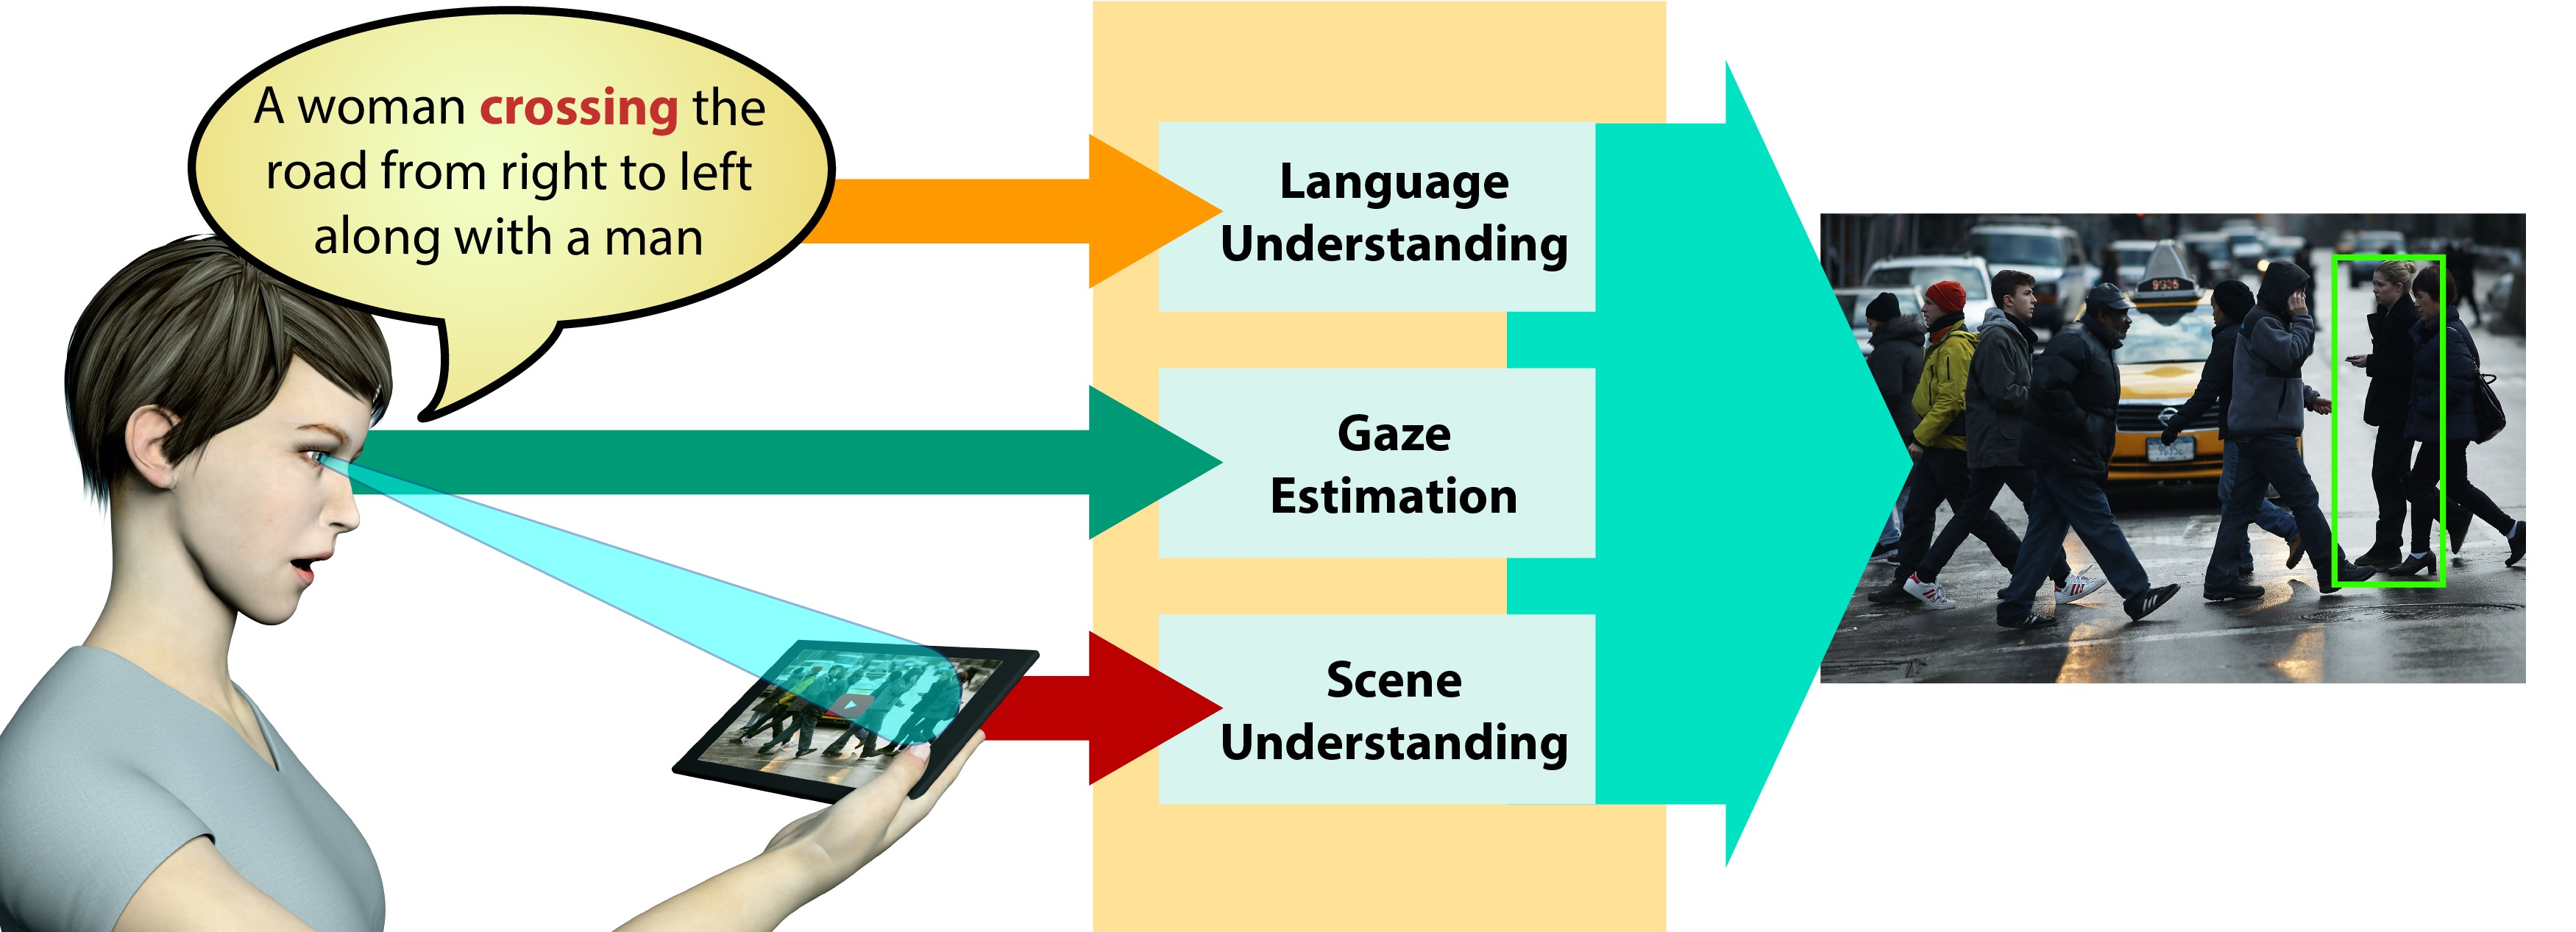
\includegraphics[width=0.47\textwidth]{teaser_w.jpg}% picture filename
   \caption{A human issuing a referring expression while gazing at the object in the scene. The system combines multiple modalities such as appearance, motion and stereo depth from the video, along with the expression and the gaze to localize the object.}
  \label{fig:teaser}
\end{figure} 


Another important cue that co-observers use to identify the objects is Gaze of the speaker. While describing the object, speakers gaze at the object to come out with an unique expression. Gaze is another important cue for object localization from the point of view of co-observer, along with the language expression. For example, suppose a car occupant instructs his/her autonomous car with expression \emph{`Park under the yellow tree on the right'}, it is highly likely that he/she is gazing at that \emph{tree}, or did so in the brief past. This gaze cue can be a promising aid to the car to localize the \emph{tree}. In this work, we also investigate how gaze can be useful in assisting the OR task. As shown in Fig.~\ref{fig:teaser}, we use text language, gaze estimates visual appearance, motion features and depth features to localize the object being referred.

%This paper investigates OR in videos with language and human gaze. 
As shown several times in computer vision, large-scale datasets can
play a crucial role in advancing research, for instance by enabling
the deployment of more complex learning approaches and by benchmarking
progress. This paper presents a video dataset for OR, the first of its
kind, with $30,000$ objects in $5,000$ stereo video sequences. The
dataset is annotated with the guidance of Gricean
Maxims~\cite{Logic:conversation} for cooperative conversations between
people.  That is, the descriptions need to be truthful, informative,
relevant, and brief for co-observers to find the target objects easily
and unambiguously. Later, human gazes are recorded as videos while
they look at the annotated objects.

\begin{figure*}[t]
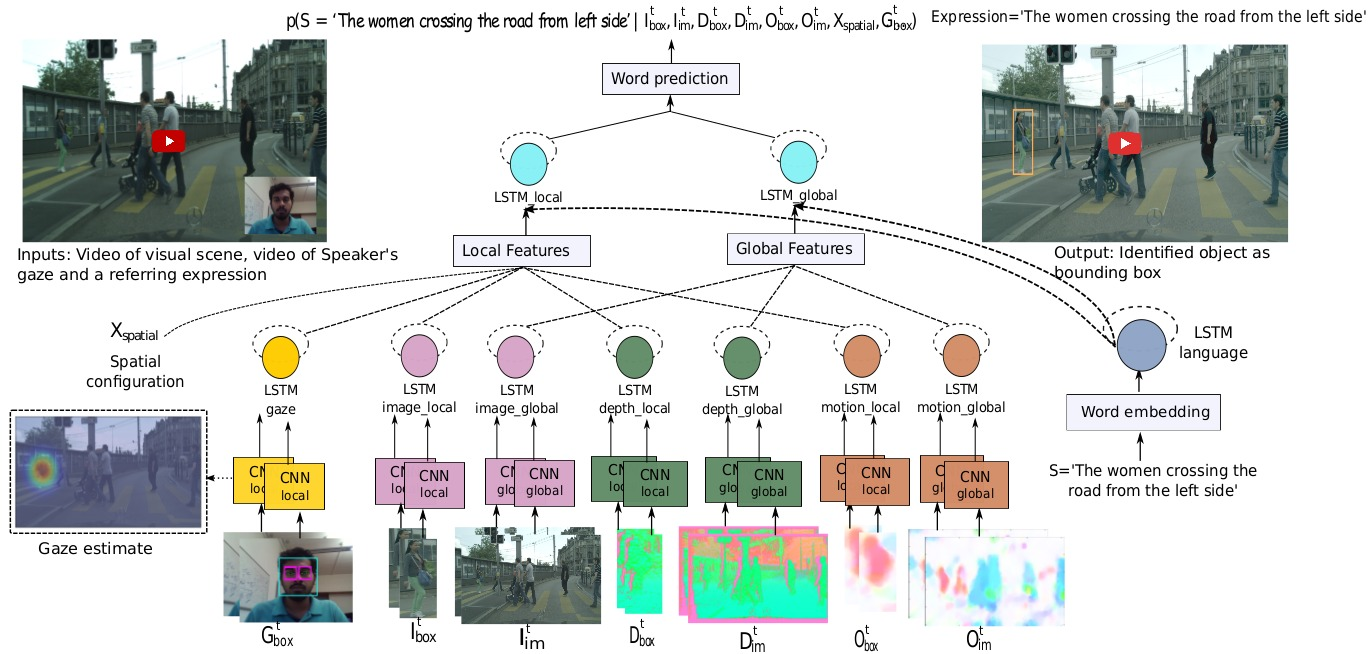
\includegraphics[width=1\linewidth]{pipeline.jpg}
\caption{The illustrative diagram of our model for object referring in
  stereo videos with language expression and human gaze. Given a
  referring expression $S$, our model scores all the $M$ bounding box
  candidates by jointly considering local appearance
  ($I_{\text{box}}^t$), local motion ($O_{\text{box}}^t$), local depth
  ($D_{\text{box}}^t$), local human gaze ($G_{\text{box}}^t$), spatial
  configuration $X_{\text{spatial}}$, and the global temporal-spatial
  contextual information ($I^t$, $D^t$ and $O^t$).}
\label{fig:pipeline}
\end{figure*}

We further propose a novel Temporal-Spatial Context Recurrent ConvNet
model, by integrating appearance, motion, gaze, and spatial-temporal
context into one network. See Fig.~\ref{fig:pipeline} for a diagram of
our model. The model learns the interactions between language
expressions and object characteristics in the `real' 3D world,
providing human users the freedom to interact by speaking and gazing.
Experimental results show that our method effectively uses motion
cues, temporal-spatial context information, and human gazes.

%Our method outperforms previous OR methods by a large margin.
%Besides temporal-spatial information to TSCRC, we conducted
%experiments by providing gaze information to TSCRC model which
%further increases the LOR accuracy.% Besides TSCRC, we present an LOD
%approach for Language-based Object Proposals.  While enjoying the
%additional information sources provided by stereo videos for LOR, the
%benefits come at a cost. Learning and inference for video LOR are
%computationally more demanding than for images. Our Language-based
%Object Proposal (LOP) method rejects irrelevant object candidates
%early and accurately. The combination of LOP and TSCRC also follows
%the procedure that human observers seem to follow to find referred
%objects: generating candidates first (often objects from the same
%class as the target object) and then using the detailed information
%in the expression for verification.  Experiments on video LOR dataset
%shows that LOP significantly outperforms expression-agnostic proposal
%techniques.
Our main contributions are: 1) presenting a new video dataset for
object referring, featuring bounding-boxes, language descriptions and
human gazes; 2) developing a novel OR approach to detect objects in
videos by learning from appearance, motion, gaze, and temporal-spatial
context.
%proposing
                                                                                                                                                                                                                                                                                            %an
                                                                                                                                                                                                                                                                                            %expression-based
                                                                                                                                                                                                                                                                                            %object
                                                                                                                                                                                                                                                                                            %proposal
                                                                                                                                                                                                                                                                                            %method.

The paper is structured as follows. Section \ref{sec:related}
summarizes relevant work. Section \ref{sec:dataset} is devoted to the
dataset, followed by Section \ref{sec:approach} for the detection
approach. Finally, Section \ref{sec:experiment} presents our
experiments. Section \ref{sec:conclusion} concludes the paper.

%Recently, the task of object retrieval from scene is getting popular among image-language tasks. This is the task of detecting a particular object based on a given text. There are number of terms associated with this task such as referring expressions \cite{yu2016modeling,mao2016generation}, phrase localization \cite{phloc,wang2016structured}, grounding of textual phrases \cite{rohrbach2016grounding}, dense captioning etc.  Referring expressions in image-language domain refer to short natural language phrases that describe an object in an image. Grounding of these expressions refers to localizing the object region in the image. 

%In this paper, we focus on grounding of natural language expressions in the image. We experiment on different proposal techniques and observe how it improves the localization of the objects in the image. Previous works dealt the problem in combined settings for object captioning and retrieval. Mao ~\etal \cite{mao2016generation} 

%------------------------------------------------------------------------

\section{Related Work}
\label{sec:related} 

Our work is relevant to the joint understanding of language and visual data. It is especially relevant to referring expression generation and language-based object detection. 

%\textbf{grounding} 
%[Grounding Verbs of Motion in Natural Language Commands to Robots]

The connection between language and visual data has been extensively
studied in the last three years. The main topics include image
captioning~\cite{deep:semantic:alignment:cvpr15, show:attend:tell,
  caption:back}, visual question answering
(VQA)~\cite{exploraing:models:data:vqa, VQA, andreas2016learning} and
referring expressions. Although the goals are different, these tasks
share many fundamental techniques. Two of the workhorses are
Multimodal Embedding~\cite{frome2013devise,
  deep:semantic:alignment:cvpr15, multimodal:pooling} and Conditional
LSTM~\cite{densecap:cvpr16, rohrbach2016grounding, yu2016modeling,
  mao2016generation}.  Multimodal Embedding projects textual data and
visual data both to a common space, in which similarity scores or
ranking functions are learned.
%A common representation space allows for discriminative learning of the interactions between the two modalities. 
Multimodal Embedding was initially explored for the task of image captioning~\cite{frome2013devise, long-term:recurrent, deep:semantic:alignment:cvpr15} and later reinforced in VQA~\cite{exploraing:models:data:vqa,ask:your:neurons,multimodal:pooling}. 
It is common practice to represent visual data with CNNs pre-trained  for image recognition and to represent textual data with word embeddings pre-trained on large text corpora~\cite{glove}. A Conditional LSTM is a generative model conditioned on visual input, and it is usually trained to maximize the generative probability of language descriptions~\cite{hu2016natural,mao2016generation} or answers to questions \cite{VQA,exploraing:models:data:vqa}. %In principle, a Conditional LSTM is more flexible and expressive, and thus more suitable for tackling open-ended language-vision problems. 
Our model conditions LSTMs not only on images but also on motion, depth and gaze.    

%\textbf{Referring Expression Generation}
%Referring expression generation is 
\bigskip
\noindent
\textbf{Language-based Object Referring.}
Language-based object referring (OR) has been tackled under different names.  
Notable ones are referring expressions \cite{yu2016modeling,mao2016generation}, phrase localization \cite{phloc,wang2016structured}, grounding of textual phrases \cite{rohrbach2016grounding}, language-based object retrieval~\cite{hu2016natural} and segmentation~\cite{hu2016segmentation}. 
Recent research foci of language based OR can be put into 2 groups: 1) learning embedding functions~\cite{multimodal:pooling,deep:semantic:alignment:cvpr15} for effective interaction between vision and language; 2) modeling contextual information to better understand a speaker's intent, be it global context~\cite{mao2016generation,hu2016natural}, or local among `similar' objects~\cite{Nagaraja2016,yu2016modeling,mao2016generation}. Our work extends \cite{hu2016natural} from static images to stereo videos to exploit richer, more realistic temporal-spatial contextual information along with gaze cues for the task of OR.  

\bigskip
\noindent
\textbf{Object Referring Datasets.} 
This section discusses relevant OR datasets:    
Google Refexp~\cite{mao2016generation}, UNC Refexp~\cite{yu2016modeling}, ReferIt~\cite{kazemzadeh2014referitgame}. 
%ReferIt is a large  dataset of referring expressions collected on TC-12 expansion of the ImageCLEF IAPR dataset ~\cite{escalante2010segmented}. 
The Google Refexp dataset, which was collected by Mao~\etal~\cite{mao2016generation}, contains $104,560$ referring expressions annotated for $54,822$ objects from $26,711$ images from the MSCOCO dataset~\cite{lin2014microsoft}. UNC Refexp was collected in the same spirit as GoogleRef, but applying the ReferIt game~\cite{kazemzadeh2014referitgame} on MSCOCO. While these datasets are large-scale and of high quality, they contain only static images. This excludes useful information about the visual scenes such as motion cues and 3D spatial configuration, and also limits the descriptions to mere appearances and 2D spatial information. We build on the success of these datasets and present a new object referring dataset for stereo videos. Annotators were encouraged to use descriptions about 3D configuration and motion cues when necessary. 

\bigskip
\noindent
\textbf{Gaze Estimation.} Gaze or eye tracking has been used in computer vision tasks like object detection~\cite{karthikeyan2013and,yun2013studying} and tracking~\cite{Vadivel_2015_CVPR}, image captioning~\cite{sugano2016seeing}, image/video annotation ~\cite{Vadivel_2015_CVPR,papadopoulos2014training,soliman2016towards} and others. Misu~\etal~\cite{misu2013situated} uses gaze and speech recorded inside a car to locate real world landmark points. Vadivel~\etal~\cite{Vadivel_2015_CVPR} uses eye tracking over videos to extract salient objects as tracklets. The task of \cite{papadopoulos2014training} matches closely with us to detect objects using gaze. Nonetheless, they use gaze to fasten the annotation for object detection. \cite{nips15_recasens} proposes to follow the gaze of people in the scene to localize the place where they look. Krafka~\etal~\cite{krafka2016eye} build an mobile application to enable large scale eye tracking annotation by crowdsourcing. Inspired from \cite{krafka2016eye}, we create a web interface to record gaze via Amazon Mechanical Turk (AMT) for object localization in videos. 

\section{Approach} 
\label{sec:approach}
Object referring (OR) is widely used in our daily communication. Here, we follow the literature~\cite{hu2016natural,mao2016generation} to formulate the problem as an object detection task. Given a video sequence of visual scene $\mathbf{I}=(I^1, I^2, ...,I^t)$ and a video sequence of speaker's gaze $\mathbf{G}=(G^1, G^2, ...,G^t)$, where $t$ is the \emph{current} frame at which the referring expression $S$ is issued, our goal is to identify the referred object $\hat{b}^t$ out of all object proposals $\{b_m^t\}_{m=1}^M$  at frame $t$. $M$ is the total number of object proposals considered. Note that we assume that $t$ is known a priori to simplify the task. In real application, the exact $t$ needs to be inferred from speaker's speech and the visual scene. The performance of our method is also evaluated at frame $t$. 



\subsection{Network Architecture} 
\label{sec:model}


% we evaluate our method on the final frame at $t$. 
% Having video frame $I^t$, a referring expression $S$, a human gaze $G$, and a set of bounding box proposals $\{b_i^t\}$ generated on $I^t$, our method is trained to identify the referred object $\hat{b^t}$ out of the proposals. 
Following \cite{hu2016natural} and the work on image captioning~\cite{densecap:cvpr16}, we choose to maximize the generative probability of the expression for the target object.   Our model is based on the Spatial Context Recurrent ConvNet  model developed in ~\cite{hu2016natural} for OR in static images. The model in~\cite{hu2016natural}  unifies three LSTMs~\cite{lstm} to integrate information from language expressions, global visual context and local object content. 
%SCRC is also similar to other image captioning and VQA models that use a CNN to represent the image, followed by an LSTM to generate the text (see \eg, \cite{long-term:recurrent, densecap:cvpr16,exploraing:models:data:vqa} ). 
%The main difference of SCRC with other image captioning and VQA models~\cite{long-term:recurrent, densecap:cvpr16,exploraing:models:data:vqa} is that SCRC accommodates also local information from the object of interest.   
 %However, it can only be applied to static images. 
%As we argued in the introduction, human perceive the world more as temporally continued snippets than as static images; human tend to describe objects by not only the appearances, but also their temporal-spatial contexts and motion features. Static images fall short in providing many of such cues. 
It has gained success in OR for static images. This work extends it so that information from stereo videos and human gazes can be incorporated, resulting in our model architecture as shown in Fig.~\ref{fig:pipeline}.

Let us denote the seven \textbf{visual} LSTM models by \model{LSTM}{gaze}, \model{LSTM}{image\_local}, \model{LSTM}{image\_global}, \model{LSTM}{depth\_local}, \model{LSTM}{depth\_global}, \model{LSTM}{motion\_local} and \model{LSTM}{motion\_global}, and their hidden states by \hstate{}{gaze}, \hstate{local}{image}, \hstate{global}{image}, ..., \hstate{global}{motion}, respectively and denote the \textbf{language} LSTM model by \model{LSTM}{language} with hidden state \hstate{}{language}. We concatenate the local and global features separately as shown in Fig.~\ref{fig:pipeline}. Successively, we have \textbf{visual-language} LSTM models namely \model{LSTM}{local} and \model{LSTM}{global} which take concatenated local and global features respectively along with \hstate{}{language} as inputs. Let us denote their hidden states as \hstate{local}{} and \hstate{global}{} respectively.
A word prediction layer is used on top of these two vision-language LSTMs to predict the words in the expression $S$. Practically, our model is trained to predict the conditional probability of the next word $w_{n+1}$ in $S$,  given the local content of the objects: $G_{\text{box}}^t$, $I_{\text{box}}^t$, $D_{\text{box}}^t$ and $O_{\text{box}}^t$, the corresponding spatio-temporal contexts: $I^t$, $D^t$ and $O^t$ as detailed in Sec.~\ref{sec:featureencod}, and all the $n$ previous words. The problem can be formulated as: 
\begin{multline}
p(w_{n+1}|w_n, ..., w_{1}, I^t, I_{\text{box}}^t, D^t, D_{\text{box}}^t, O^t, O_{\text{box}}^t, G_{\text{box}}^t) \\
= \text{SoftMax}(W_{\text{local}}\vect{h}_{\text{local}}(n) + W_{\text{global}}\vect{h}_{\text{global}}(n) + \vect{r})
\end{multline}
where $W_{\text{local}}$ and $W_{\text{global}}$ are the weight matrices for word prediction from \model{LSTM}{local} and \model{LSTM}{global}, and $\vect{r}$ is a bias vector.  

At training time, the method maximizes the probability of generating all the annotated expressions over the whole dataset. Following \cite{hu2016natural}, all the seven LSTM models have $1000$ hidden states. 
At test time, given a video sequence $\mathbf{I}$, a gaze sequence $\mathbf{G}$ and $M$ candidate bounding boxes $\{b_m^t\}_{m=1}^M$ at frame $t$ considered by the method proposed in Sec.~\ref{sec:objprop}, our model computes the OR score for $b_m$ by computing the generative probability of $S$ on $b_m^t$(box):
\begingroup\makeatletter\def\f@size{8}\check@mathfonts
\begin{multline}
s_i=p(S|I^t, I_{\text{box}}^t, D^t, D_{\text{box}}^t, O^t, O_{\text{box}}^t, G_{\text{box}}^t) \\
=\prod_{w_n \in S}{p(w_n|w_{n-1}, ..., w_1, I^t, I_{\text{box}}^t, D^t, D_{\text{box}}^t, O^t, O_{\text{box}}^t, G_{\text{box}}^t ).} 
\end{multline}
\endgroup
The candidate with the highest score is taken as the predicted target object. Below, we describe our object proposal and feature encoding. 

\subsection{Object Proposals}
\label{sec:objprop} 

%One straightforward approach to Object Referring (OR) would be to train a model to directly predict the bounding box location given the gaze and the referring expression (and image). However, this will be prohibitively expensive to compute. 
In the spirit of object detection, we adopt the strategy of proposing candidates efficiently and then verifying the candidates with a more complex model for the OR task. This strategy has been used widely in the literature. For instance, \cite{hu2016natural} uses EdgeBox~\cite{ZitnickECCV14edgeBoxes} for the object proposals;  
\cite{mao2016generation} and \cite{deep:semantic:alignment:cvpr15} use the faster RCNN (FRCNN) object detector \cite{renNIPS15fasterrcnn}, Mask-RCNN~\cite{he2017mask} and Language based Object Proposals (LOP)~\cite{vasudevan2017chi} and others to propose the candidates. 
%It has been shown that using proposals strikes a good trade-off between accuracy and speed. 
\cite{vasudevan2017chi} shows that LOP performs significantly better than other techniques when we propose expression-aware object candidates. For the same reason, we use LOP~\cite{vasudevan2017chi} for the object proposals.
% \begin{algorithm}
%  \KwData{Image($I$), Disparity map($D$), Flow($O$), Gaze Video($G$), Referring Expression($S$)}
%  \KwResult{Object Detection }
%   Object Proposals: $b_{i}, \{i=1,2,3,...\}$ \\
%   $f^{local}_{image} = VGG(I_{b})$\cite{vgg16}\;
%   $f^{global}_{image} = VGG(I)$\;
%   $f^{local}_{depth} = HHAmodel(D_{b})$\cite{rgbd:net:eccv14}\;
%   $f^{global}_{depth} = HHAmodel(D)$\;
%   $f^{local}_{motion} = flow(O_{b})$\cite{two:stream:nips14}\;
%   $f^{global}_{motion} = flow(O)$\;
%   $h_{language} = LSTM_{language}(S)$\;
%   $gaze= GE(G)$\;
%  \While{For all bounding box $b_{i}$}{
%  \begin{multline}
%   score_{i}=NLOR(f^{local}_{image}, f^{global}_{image}, f^{local}_{depth}, \\ f^{global}_{depth}, f^{local}_{motion}, f^{global}_{motion}, h_{language}, f_{spacial})\;
%   \end{multline}
%  }
%  Detected box: $b_{argmax(score_{i})}$\;
%  \caption{Overall approach}
% \end{algorithm}

% \begin{algorithm}
%  \KwData{Gaze of corners $G_{1}$, $G_{2}$, $G_{3}$, $G_{4}$ and Corners(image coordinates) $I_{1}$, $I_{2}$, $I_{3}$, $I_{4}$}
%  \KwResult{Gaze Features($F$) }
%  Corners (camera coordinates) $C_{1}$, $C_{2}$, $C_{3}$, $C_{4}$\;
%   $C_{i} = DAN(G_{i})$\;
%   $I_{i} = A*C_{i} +B$ where $A=(a1, a2)$ and $B = (b1, b2)$\;
%   Solve for A and B\;
%  \While{For all Gaze $g_{i}$ and bounding box $BB_{i}$}{
%   $p_{i}= A*DAN(g_{i}) +B$\;
%   $heatmap=gaussian\_2d(Image,p_{i},\sigma=20)$\;
%   \eIf{$p_{i}$ within image}{
%    $F_{i}=mean(heatmap[BB_{i}])$\;
%    }{
%    $BB\_norm = heatmap[BB_{i}]/max(heatmap[BB_{i}])$
%    $F_{i}=mean(BB\_norm)$\;
%   }
%  }
%  Gaze Features= F\;
%  \caption{Extracting Gaze Features}
% \end{algorithm}

\subsection{Feature Encoding}
\label{sec:featureencod} 
In order to better use the spatio-temporal information provided by a stereo video, we augment $I^t$ with the corresponding depth map $D^t$ and optical flow map $O^t$. In addition to these global contexts, for a bounding box $b^t$, its local features are used as well: $I_{box}^t$ for its appearance, $D_{box}^t$ for its depth characteristics, $O_{box}^t$ for its motion cues and $G_{box}^t$ for the gaze. CNNs are used to encode the local and global information from the three information sources. $I_{box}^t$, $D_{box}^t$ and $O_{box}^t$ can be computed on frame $t$ alone or together with multiple previous frames for long-range temporal interaction. The same is applicable for $I^t$, $D^t$ and $O^t$ also. The detailed evaluation can be found in Sec.\ref{sec:experiment}.  

\noindent \textbf{Appearance.}
We use the \emph{fc7} feature of VGG-16 net~\cite{vgg16} pre-trained on ILSVRC-2012~\cite{imagenet:2015} to represent $I_{box}^t$ and $I^t$, which are passed through \model{LSTM}{image\_local} and \model{LSTM}{image\_global} respectively to yield features $\vect{f}_{local}^{image}$ and $\vect{f}_{global}^{image}$, respectively.

\noindent \textbf{Depth.}
For depth, we convert depth maps to HHA images~\cite{rgbd:net:eccv14} and extract the CNN features with the RGB-D network of ~\cite{rgbd:net:eccv14} before passing to \model{LSTM}{depth\_local} and \model{LSTM}{depth\_global}. This leads to  depth features $\vect{f}_{local}^{depth}$ and $\vect{f}_{global}^{depth}$ for $D_{box}^t$ and $D^t$, respectively. 

\noindent \textbf{Optical Flow.}
Similarly, we employ the pre-trained two-stream network~\cite{two:stream:nips14} trained for video action recognition to extract convolutional flow features. Again, the \emph{fc7} features are used leading to $4096$-dimensional features which are given to \model{LSTM}{motion\_local} and \model{LSTM}{motion\_global} to get the motion features $\vect{f}_{local}^{motion}$ and $\vect{f}_{global}^{motion}$ for $O_{box}^t$ and $O^t$. 

\noindent \textbf{Language.} 
The words in the expression $S$  are represented as one-hot vectors and embedded by word2vec~\cite{glove} first and later, the expression $S$ is embedded by an LSTM model~\cite{lstm} \model{LSTM}{language}, leading to a language feature vector $\vect{h}^{\text{language}}$ for $S$.  

\noindent \textbf{Human Gaze.}
We synchronize the video of human gaze and the Cityscapes's video, which was displayed on a laptop for gaze recording. On the extracted frames, we perform face detection to crop out the face image and then conduct facial landmark point detection using the work of \cite{kowalski2017deep}. Successively, we detect the left eye and the right eye, and extract them as well. An example is shown in Fig.~\ref{fig:pipeline}. Then, we use GazeCapture model~\cite{krafka2016eye} which takes input of left and right eye images along with the face image and outputs the gaze estimates relative to the camera location on the device. We convert the estimate from camera coordinate system to image coordinate system by applying a linear mapping function. The mapping function is device-specific and defined by the relative position of the camera and the screen of the laptop. More details of the mapping function can be found in the supplementary material. 
%Once we have the mapping function which is particular for a device and position of canvas on the screen where we are supposed to gaze, we can obtain the gaze in image coordinates frame-by-frame for the entire gaze recording video.

%We extract the gaze features by aggregating the feature from each frame of the gaze video. 
%For each frame of the video, we estimate the image coordinates where gaze is focused on the image canvas. 
Finally, we plot a 2D Gaussian map around the estimated gaze coordinates on the image to accommodate the errors in gaze estimation by the GazeCapture model~\cite{krafka2016eye} as shown in Fig.~\ref{fig:gaze_error}. Later, we compute gaze feature for an object in a frame by region pooling (averaging) over the bounding box region inside the Gaussian map. We concatenate these features over all the frames of the video to yield a resultant gaze feature $\vect{f}^{gaze}$ for an object~\ie $G_{box}^t$.


\noindent \textbf{Feature Concatenation.}
Similar to \cite{hu2016natural}, we concatenate the language feature with each of the two concatenated local and global features to obtain two meta-features: $\{[\vect{h}^{\text{language}}, \vect{f}_{local}^{image}, \vect{f}_{local}^{depth}, \vect{f}_{local}^{motion}, \vect{f}^{gaze},\vect{f}_{spatial}]$, $[\vect{h}^{\text{language}}, \vect{f}_{global}^{image}, \vect{f}_{global}^{motion}, \vect{f}_{global}^{motion}]\}$. The meta-features are then given as the input to two LSTM models \model{LSTM}{local} and \model{LSTM}{global} respectively, to learn the interaction between language and all the `visual' domains, \ie appearance, motion, depth, gaze and their global contexts.  
$\vect{f}_{spatial}$ denotes the spatial configuration of the bounding box  with respect to the 2D video frame. Following~\cite{mao2016generation,hu2016natural}, this $8-$dimensional feature is used:  
\begin{equation}
\vect{f}_{\text{spatial}}=[x_{\text{min}}, y_{\text{min}}, x_{\text{max}}, y_{\text{max}}, x_{\text{center}}, y_{\text{center}}, w_{\text{box}}, h_{\text{box}}]
\end{equation}
where $w_{\text{box}}$ and $h_{\text{box}}$ are the width and height of the box. 
%$\vect{f}_{\text{spatial}}$ is added to the augmented local image features.%, leading to a new feature $[\vect{h}_{\text{language}}, \vect{f}_{image}^{local}, \vect{f}_{\text{spacial}}]$ for the model \model{LSTM}{image\_local}. 
See Fig.~\ref{fig:pipeline} for all the interactions. Our method can be trained in a full end-to-end fashion if enough data is provided.  

\begin{figure}[t]
\centering
\begin{tabular}{lll}
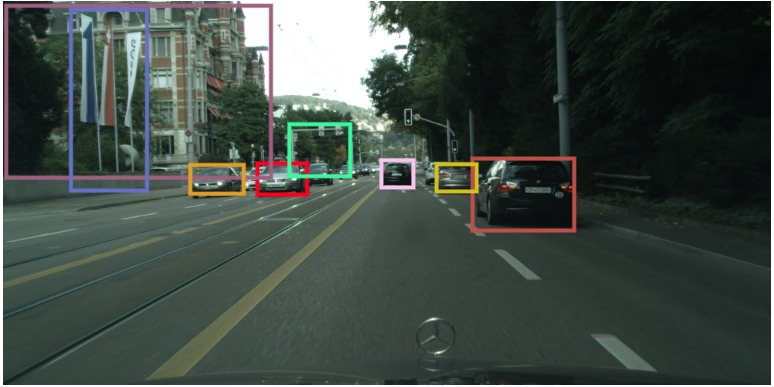
\includegraphics[width=0.5\linewidth]{pic5.jpg}
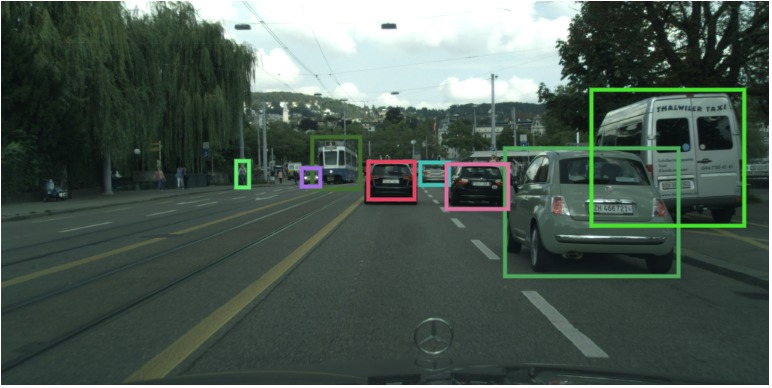
\includegraphics[width=0.5\linewidth]{pic6.jpg}
\noindent 
\noindent
%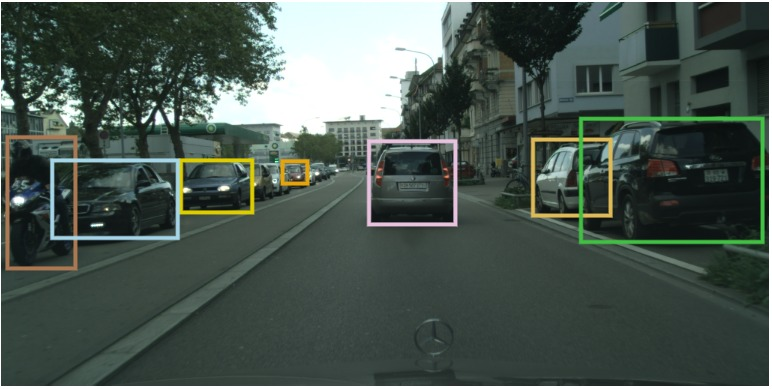
\includegraphics[width=0.23\linewidth]{figures/pic3.jpg}
%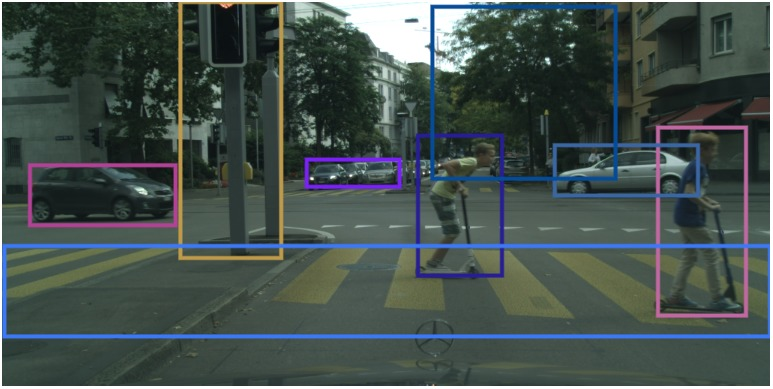
\includegraphics[width=0.23\linewidth]{figures/pic4.jpg}
\\
\noindent 
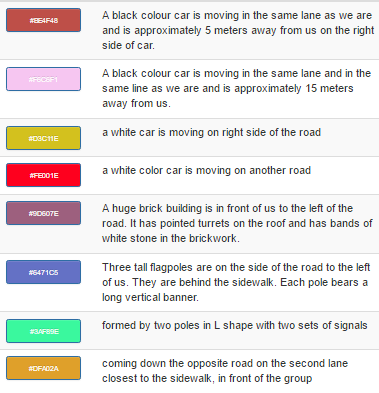
\includegraphics[width=0.5\linewidth,height=0.50\linewidth]{desc5.PNG}

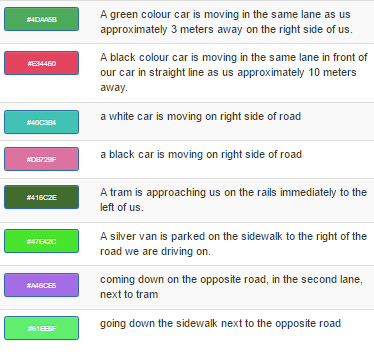
\includegraphics[width=0.5\linewidth,height=0.50\linewidth]{desc6.PNG}
%\noindent 
%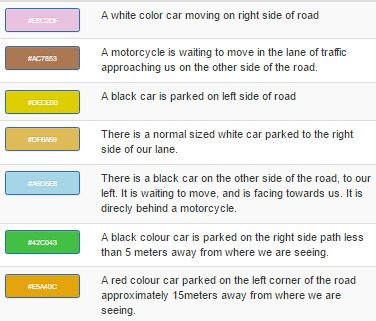
\includegraphics[width=0.23\linewidth,height=0.20\linewidth]{figures/desc3.jpg}
%\noindent 
%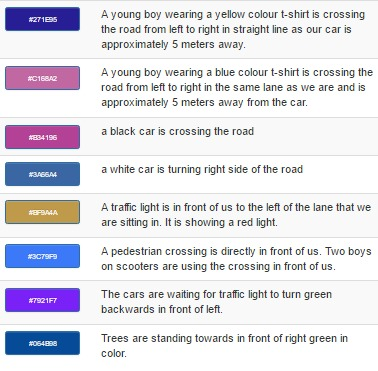
\includegraphics[width=0.23\linewidth,height=0.20\linewidth]{figures/desc4.jpg}

\end{tabular}
\caption{Top: sample images from the Cityscape dataset with objects marked in differently colored bounding boxes. Bottom: corresponding referring expression annotations.}
\label{fig:recallvsiou}
\end{figure}

%We first evaluate the accuracy of the class association by our LSTM model. On the GoogleRef dataset, it achieves an accuracy of 90.5\% on the validation set. On the Cityscapes dataset, it achieves 91.5\% on the validation set. The high accuracy of the class association implies that expression-based object proposing is promising.  
%Due to this high accuracy, it is reasonable to define the \emph{relevant} classes as those with the highest association scores. 
%We take the most confident one as the  \emph{relevant} class and the rest as \emph{irrelevant} ones. Given all the detection candidates from the FRCNN detector, we use our LSTM association model to filter out all the detections from the \emph{irrelevant} classes, and only pass those from the \emph{relevant} class to the subsequent language-model for the final selection. 

%It is better to use a LSTM than simply taking the first noun to find the \emph{relevant} class. This is because LSTM can capture high level semantics and contextual information from the textual description such as actions or events that may reflect some particular class.~\eg driving is more likely to refer to a \emph{car/person} than a \emph{building}.
%using GoogleRef training set comprising of $85474$ referring expressions for objects. The output layer has $80$ nodes for 80 categories of MSCOCO. The output layer is passed through a softmax non-linearity. 

%%\dengxincomment{explain why it is better than simply taking the first noun? due to context, \eg in actions and motion features can also reflect the classes. driving is about car, riding is about bicycles. } 
%\subsection{ReferIt}
%\subsection{Cityscape}


%It is highly likely that salient objects are ranked higher than any typical object in the image. The ranking of the object proposals can be ranked based on the objects mentioned in the expression. 

%We see that FRCNN object detections are agnostic to the referring expressions. Ranking of the proposals are based only on the detection score. It is highly likely that salient objects are ranked higher than any typical object in the image. The ranking of the object proposals can be ranked based on the objects mentioned in the expression. We learn a two  layer LSTM with 300 hidden layer nodes each using GoogleRef training set comprising of $85474$ referring expressions for objects. The output layer has $80$ nodes for 80 categories of MSCOCO. The output layer is passed through a softmax non-linearity. LSTM is trained to get 90.5\% validation accuracy on the text classification.

%follow the literature to adopt a simpler, ranking-based approach. The reason behind this choice is that .... 

%Because, ... we develop a new approach consisting of two steps: language-based object proposal and   



%\subsection{Detection model}
%\label{detectionmodel}


%s_i=p(S|I, I_{\text{box}}, D, D_{\text{box}}, O, O_{\text{box}) 
%

%\dengxincomment{ Deep Multimodal Similarity Model or generative model?}
%c.f. From Captions to Visual Concepts and Back


\section{Dataset Annotation}
\label{sec:dataset}

As discussed in Sec.~\ref{sec:intro} and Sec.~\ref{sec:related}, previous datasets do not cater to the learning and evaluation of temporal, spatial context, and gaze information.  Thus, we collected a new dataset.  A video OR dataset should contain  diverse visual scenes and their objects should be annotated at the frame (time) when the expression is issued. We acknowledge that all modalities should be recorded/annotated at the same time, ideally in the real human-to-robot communication scenarios. That, however, renders data collection very labor-intensive and infeasible to crowd source.  

In this work, we choose to use the existing stereo videos from Cityscapes dataset~\cite{cityscape}, and annotate language expressions, object bounding boxes, and gaze recordings via crowd sourcing. Cityscapes consists of $5,000$ high-quality video sequences in total, captured with a car mounted stereo camera system in $50$ different European cities.  The videos contain diverse sets of traffic scenes such as \emph{car approaching a signal stop}, \emph{pedestrians crossing the road}, \emph{trams running through the street}, and \emph{bicycles are overtaken}, and \emph{kids crossing  road lanes}, \etc. See Fig.~\ref{fig:recallvsiou} for some examples.

% A good dataset needs to be challenging, but at the same time it should be accessible to the current learning approaches. 
% Imposing this constraint helps the learning algorithm to effectively exploit the enriched spatio-temporal information on a reasonably large dataset. The enriched information leads to larger variations of data samples, which in turn require a very large dataset for learning if no constraint is imposed to the data type. Another reason for this choice is the availability of the excellent Cityscapes dataset. 

%Our dataset is also collected for referring expressions for objects in images and the way of data collection allows our referring expressions to have both spatial and temporal information of objects. e.g. car is slowing down for the signal.


%in train set and $500$ videos in validation set. The videos in the dataset are captured from the interior of a car which drives around $50$ different cities. The videos generally captures diverse set of road scenes such as car approaching to a signal stop, pedestrians crossing the road, trams, bicycles, cars crossing our road lanes, etc. We annotated the referring descriptions for each object in the scene. This helps not only in the semantic understanding of the scene but also in carrying out an informative communication between human and car.

\bigskip
\noindent
\textbf{Crowdsourcing}. We crowdsourced the annotation task of OR in videos via AMT. Each Human Intelligence Task (HIT) contains one video.
%with five assignment tasks, for five different worker. 
The videos in the Cityscapes dataset are all 2 seconds long, comprising 30 frames. An AMT worker was asked to annotate bounding boxes for objects on the last frame of the video (\ie the 30th frame). The 30th frame is chosen mainly to  make sure that annotated objects come with sufficient temporal context. In the annotation, workers are `forced' to watch the video at least once in order to annotate an object. Replaying the video is highly encouraged if something is unclear. 
%The dataset is annotated under the guidance of  Gricean Maxims~\cite{Logic:conversation} for cooperative conversation between people.  Workers are asked to give truthful, informative, relevant, and brief expressions so that co-observers, or later an autonomous car, can find the referred objects easily and unambiguously.  
%For each annotated object, the frame id is fixed as the 30th frame of the videos. Our aim of our dataset is to improve the system of LOD at the frame level using spatio-temporal information from the videos. Hence, we focus on the annotation of objects on a fixed video frame rather than on the whole set of frames.

\bigskip
\noindent
\textbf{Quality Control}. To generate high quality annotations, we ran the first round of HIT as a qualification task. We qualified 20 workers based on their annotation of bounding boxes and natural language descriptions who further annotated the entire dataset. %The annotations are also manually checked to spot erroneous annotations. 
Following the work of Li~\etal \cite{li2016tgif}, we employed various quality control mechanisms for the syntactic validation to ensure the high quality of sentences. Some of the used validation checks are: number of words in the description must be at least 5, words must contain only ASCII characters, copy/paste operation is not allowed in the field where workers typed the descriptions and finally, we check for grammatical and spelling errors using the HTML5 spellcheck attribute. We payed $0.075$ US dollar for each annotation of one bounding box, the name of the object class, and a referring expression. In total, we have collected $30,000$ annotated objects in $5,000$ videos.  %The annotation interface will be provided in the supplementary material. 

\bigskip
\noindent
\textbf{Dataset Statistics}. The average length of referring expressions of the objects is $15.59$ words compared to $8.43$ in Google Refexp and $3.61$ in the UNC Refexp dataset, which are popular referring expression datasets. 
%Our expressions are richer mainly because the scenes are more complex and the speakers (Workers) need to distinguish the referred object from other traffic agents. 
There are 20 classes of objects in Cityscape. The average number of referring expressions on objects annotated per image is $4.2$ compared to $3.91$ in Google Refexp. The distribution of annotations is 53.99\% referring expressions for 'car', 22.97\% for 'person', 4.9\% for 'vegetation', 3.9\% for 'bicycle', 3.46\% for 'building', 2.95\% for 'rider' and the rest for the remaining categories. %There was a large difference in the number of annotations for each object.

\bigskip
\noindent
\textbf{Gaze Recording}. As a separate annotation task, We record human gaze for the objects which have been annotated already with referring expressions and bounding boxes. This is inspired from Krafke~\etal \cite{krafka2016eye} where eye tracking dataset is created via crowdsourcing by asking workers to gaze at particular points on the device screen with their face being recorded. Here, we collect the gaze recording on objects annotated in Cityscapes dataset as mentioned beforehand in this section. We create a web interface where we show the videos and asked the turk workers to gaze at the object one after the other. We record the faces of workers using the frontal camera of their laptops while they gaze at the shown objects.

In our annotation interface, we instruct the workers to adjust the window size such that the canvas where videos are displayed, occupies a major amount of screen space for a higher resolution of gaze estimation. 
% This helps in capturing better differences in the gazes even when the objects are close in the video.
With the start of the annotation, workers are asked to watch the complete video at first to put them into context.
% Once video is ended, workers are instructed to click at the highlighted corners of the canvas and gaze of the worker is captured at the instant they click. This ensures that we capture the gaze of the workers on the corners which we later use for the calibration. Corner gazes are used to compute the mapping function from camera coordinates to image coordinates as mentioned in Sec.~\ref{sec:approach}. This is important because 1) Workers may use devices with different dimensions, 2) Window of the interface may not be of full screen in their device. Once all corners are clicked, 
Once this is done, we show the objects (in bounding boxes) with annotated bounding boxes on the canvas. The workers are asked to click inside the box which activates the running of the video. 
%Since the bounding box clicking happens at the last frame of the video, we reverse the video till the 10th frame from the last and then resume the video. We use 10 frames which acts as a tradeoff between the length of the video streamed for gazing and the time for which the object is still in image context.
We direct the workers to gaze at the same clicked object during the stage of video streaming while we recording the gaze of the worker throughout this period. Successively, we show the next objects and record the gazes correspondingly. 
%They are allowed to submit the task once all the objects are gazed. 4 gaze recorded images for the corners and 
At the end of the annotation of each video, we collect a video for the gaze recording of every annotated object.

We ensured the quality of recording by allowing only qualified workers to participate in this task. We perform the qualification same as in the earlier task except the criteria being checked is gazing here. Workers perform the task under different lighting conditions and at times, their visibility of their face goes down with its consequence being that the face detection fails in those cases. Hence, we re-recorded the gazes for all the videos where face detection on the workers failed. Finally, we recorded gaze for all the annotated objects of the Cityscapes.


%\dengxincomment{remember to mention that for this dataset, the frame id of the object is fixed and given. justify this. it is not a full system of LOD in videos. }

%\section{Multiple Modalities}
%\dengxincomment{generate audio?}

%\section{Object Proposal}\label{sec:objprop}

%In the object detection tasks, it is intuitive that the quality of the object detection depends on the candidate proposal quality. Edgebox(sliding window approach) \cite{ZitnickECCV14edgeBoxes}, Selective Search \cite{van2011segmentation}, MCG \cite{arbelaez2014multiscale} (grouping superpixels) and among others are few of the widely used object proposals technique. Further, these bottom up region proposals along with features from Region based CNN (RCNN) are used for the object detection. Current state of the art object detection uses two modules - Region Proposal Network for region proposal and Faster RCNN for object category classification \cite{renNIPS15fasterrcnn}. 

%\bigskip
%\noindent
%\textbf{FRCNN object detection}. In our baseline model, Hu ~\etal \cite{hu2016natural} uses Edgebox for the region proposals. These EdgeBox proposals are used as candidates for object and each candidate is scored based on the given natural language expression, similar to image-language tasks. We investigate on different techniques to improve the object proposals. Since our task is to retrieve objects from the image based on a given text, object proposals should be more object centric. We use Faster RCNN (FRCNN) with RPN for object proposals, which is pre-trained on MSCOCO for object detection task. Each of the object proposal is output with a detection score. Unlike a threshold used by \cite{renNIPS15fasterrcnn}, we keep constraint on the total number of detections to be $100$. Thus, we have $100$ region proposals for the subsequent Natural language object retrieval (NLOR) model.

%\bigskip
%\noindent
%\textbf{Re-Ranking Proposals}. We see that FRCNN object detections are agnostic to the referring expressions. Ranking of the proposals are based only on the detection score. It is highly likely that salient objects are ranked higher than any typical object in the image. The ranking of the object proposals can be ranked based on the objects mentioned in the expression. We learn a two  layer LSTM with 300 hidden layer nodes each using GoogleRef training set comprising of $85474$ referring expressions for objects. The output layer has $80$ nodes for 80 categories of MSCOCO. The output layer is passed through a softmax non-linearity. LSTM is trained to get 90.5\% validation accuracy on the text classification.





\section{Experiments}
\label{sec:experiment}

Given a video sequence of visual scene, gaze recording sequence of the speaker and a referring expression, our task is to yield bounding box location of the object. 
%Our entire pipeline can be seen as two parts: a) a TSCRC model using three data modalities: RGB, depth and motion; b) a Gaze Prediction model, both assist for language-based object referring (LOR). 
Our model scores and ranks the object proposals (which we generate using LOP~\cite{vasudevan2017chi}) based on the textual description, the spatial and temporal contextual information from stereo videos and gaze recording of the speaker. We first evaluate the performance of multiple modalities namely, RGB image, depth information and object motion. It is aimed to show the usefulness of depth and motion provided by stereo videos for the task of Object Referring (OR). Later, we show how gaze aids our model to improve the OR accuracy further.

\subsection{Implementation Details}
Our model is designed to incorporate gaze of the speaker, temporal and depth cues of the objects as well as the contextual information. The main advantage of Cityscapes referring expression annotations over other referring expressions datasets like GoogleRef, UNC Refexp and ReferIt is that the Cityscapes consists of short video snippets and the corresponding depth maps, suited for our task. For RGB images, we extract features from VGG16~\cite{vgg16} as mentioned in Sec.~\ref{sec:approach}. For depth, we generate HHA images from disparity maps following the work of Gupta~\etal~\cite{rgbd:net:eccv14}. Furthermore, we extract HHA features using the RCNN network used by \cite{rgbd:net:eccv14}. For motion, we compute optical flow for all the frames using Fast Optical Flow by Kroeger~\etal~\cite{kroeger2016fast}. We extract optical flow features using the flow network of the two stream Convolutional network implemented by Simonyan~\etal~\cite{two:stream:nips14} for action recognition in videos. To compute object level features in all frames of videos, we compute tracks of the objects using the annotated bounding box on the last frame of the videos(30th frame in Cityscapes). We compute tracks for each object using Correlation filter based tracking~\cite{valmadre2017end}. 

Coming to Gaze, we sample frames from gaze video at a frame rate greater than frame rate of gazed Cityscapes video to ensure one-to-one correspondence between the sequences. Then, we extract the face image from each of the frame using Face Detection using Haar Cascades~\cite{viola2001rapid}. For these face images, we use Deep Alignment Network~\cite{kowalski2017deep} to extract facial landmark points. Using the left and right eye landmark points, we extract the left and right eye image which we later give to GazeCapture model~\cite{krafka2016eye} along with face information. GazeCapture model outputs the gaze prediction in camera coordinates. We convert these camera coordinates to image coordinates using the linear mapping function as mentioned in Sec.~\ref{sec:approach}. 
%Thus, Gaze estimation system, as a whole, gives the prediction in image coordinates given the face image and gaze recording on the corners of the image. 
Then, we plot 2D Gaussian plot around the gaze estimate in image coordinates with $\sigma=100$ pixels which is 10\% of image dimension. This helps in accommodating the prediction error of gaze coordinates from the GazeCapture model as mentioned in ~\cite{krafka2016eye}. See Fig.~\ref{fig:gaze_error} for gaze prediction error distribution. Successively, we perform region pooling over the bounding box location of Gaussian map to obtain the object feature. We concatenate the features from each frame to get the gaze feature for the entire recording. Finally, we train our model by using the extracted features from RGB, HHA, Optical Flow images and gaze features as shown in Fig.~\ref{fig:pipeline}.

%-----------------------------------------------------------------------
\begin{table}[t]
\centering
\resizebox{0.9\columnwidth}{!}{
\begin{tabular}{@{}lllllllllllll@{}}
\toprule
 %&            & \multicolumn{2}{c}{HIT @ 1} &   &         \\ \cmidrule{3-4}
 &Methods &\multicolumn{1}{c}{Edgebox}&\multicolumn{1}{c}{FRCNN} &\multicolumn{1}{c}{LOP }\\
% \cmidrule(lr){1-2} \cmidrule(lr){3-3} \cmidrule(lr){4-6}  \cmidrule(l){7-9}
% &Candidate Proposals &\multicolumn{1}{c}{100} &\multicolumn{1}{c}{10} &\multicolumn{1}{c}{30}&\multicolumn{1}{c}{100 }& \multicolumn{1}{c}{10 }  & \multicolumn{1}{c}{30 } & \multicolumn{1}{c}{100 }      \\ 
% \cmidrule(lr){1-2} \cmidrule(lr){3-3} \cmidrule(l){4-5}\cmidrule(l){6-7} \cmidrule(l){8-10}\cmidrule(l){11-13}
%&Method         &Acc@1 &  Acc@1  &  Acc@5 &Acc@1  &  Acc@10 & Acc@1 &  Acc@10  &  Acc@30  & Acc@1 &  Acc@10  &  Acc@100    \\ 
\midrule
%\multicolumn{10}{l}{\textsc {GoogleRef}}   \\
%& Random &0.98& 3.75& -  \\
%& NLOR \cite{hu2016natural} & 9.02& -&25.04& -&36.1& -& -&? & 15.01 & 50.61& 73.78 \\
& SimModel \cite{phloc}&4.5& 18.431& 35.556 \\
& NLOR \cite{hu2016natural}(Ours(I)) &4.1& 27.15& 36.895 \\
%& Mao ~\etal \cite{mao2016generation}  & 17.5 & - &- \\
& Ours (I,D) & -&38.562& 40.948  \\
& Ours (I,O) & -&38.856& 42.255  \\
& Ours (I,D,O) & -& 39.509& 43.137  \\
& Ours (I,D,O,G) & -& \textbf{45.784}& \textbf{45.065}  \\

\bottomrule
\end{tabular}
}
\caption{Numbers denote Acc@1. The \# of candidate proposals $M$ is $30$. All evaluations are on Cityscapes. Abbreviations: I:RGB, D:Depth map, O:Optical Flow, G:Gaze. Since Edgebox performs poorly in baseline:Ours(I), we avoid further experiments.}
\label{tab:eop-expt}
\end{table}


% \begin{table}[t]
% \resizebox{1.0\columnwidth}{!}{
% \centering
% \begin{tabular}{@{}lllllll@{}}
% \toprule
%  %&            & \multicolumn{2}{c}{HIT @ 1} &   &         \\ \cmidrule{3-4}
%  &Candidate Proposals & \multicolumn{1}{c}{10 }& \multicolumn{3}{c}{30 }             \\ 
%  \cmidrule(lr){1-2} \cmidrule(lr){3-3} \cmidrule(l){4-6}
% &Method       & Acc@1   & Acc@1 &  Acc@10  &  Acc@30   \\ \midrule
% %\multicolumn{10}{l}{\textsc {GoogleRef}}   \\
% %& Random&- &  5.87& -&-  \\%5.87 & 36.49  \\
% & NLOR \cite{hu2016natural}(SCRC+EdgeBox)&15.88 & 16.86& 47.38&55.70 \\% 16.51 & 52.45 \\

% %& NLOR \cite{hu2016natural} & -& 14.24&25.04& 15.88&36.10& 16.86& 47.38&? & ? & ?& 73.52 \\
% %& Mao ~\etal \cite{mao2016generation}  & 17.5 & - &- \\
% %& Sim model(embedding)+frcnn & -&- & - & - & -   \\
% %& Sim model(rankloss)+frcnn& -& 29.38& 66.92& -&77.26& -& -&- & - & 55.24 & -   \\
% & Sim model~\cite{karpathy2014deep}+FRCNN&27.06& 19.62&76.35 & 87.78 \\%& 14.25 & 55.24   \\
% & MCB~\cite{fukui16mcb} &31.24 &28.34& 78.76 &87.78  \\
% & SCRC+FRCNN&38.28 & 31.9& 79.33&87.78  \\%24.77 & 68.47 \\
% %& Similarity model+frcnn-lstm& -& 23.00& 49.07& 21.24&61.11& -& -&- & - & 55.24 & -   \\
% & SCRC + LOP &\textbf{42.11}& \textbf{38.42}& \textbf{83.27}&\textbf{87.78} \\%& 32.72 & 83.78 \\
% \bottomrule
% \end{tabular}
% }
% \caption{Acc@K represents the accuracy of grounding of referring expressions on objects with IoU=$0.5$. The different methods are evaluated on GoogleRef.}
% \label{tab:googleref}
% \end{table}



% \begin{table}[t]
% \resizebox{1.0\columnwidth}{!}{
% \centering
% \begin{tabular}{@{}llllllll@{}}
% \toprule
%  %&            & \multicolumn{2}{c}{HIT @ 1} &   &         \\ \cmidrule{3-4}
%  &Candidate Proposals & \multicolumn{1}{c}{10 }&\multicolumn{2}{c}{30 }         & \multicolumn{2}{c}{100 }      \\ 
%  \cmidrule(lr){1-2}\cmidrule(lr){3-3} \cmidrule(lr){4-5} \cmidrule(l){4-5}\cmidrule(l){6-7}
% &Method         & Acc@1 &  Acc@1  &  Acc@10  & Acc@1 &  Acc@10   \\ \midrule
% %\multicolumn{10}{l}{\textsc {GoogleRef}}   \\
% %& Random &  -& -&- & 1.5 &8.57  \\
% & NLOR \cite{hu2016natural} &2.15& 4.1& 10.06 & 7.8 & 18.85 \\
% & SCRC+FRCNN &25.49& 27.15& 70.58 & 20.26 & 58.16 \\
% %& NLOR \cite{hu2016natural} & -& 14.24&25.04& 15.88&36.10& 16.86& 47.38&? & ? & ?& 73.52 \\
% %& Mao ~\etal \cite{mao2016generation}  & 17.5 & - &- \\
% %& Sim model(embedding)+frcnn & -&- & - & - & -   \\
% %& Sim model(rankloss)+frcnn& -& 29.38& 66.92& -&77.26& -& -&- & - & 55.24 & -   \\
% %& Sim model(classify)+frcnn& -&- & - & - & -   \\
% %& Similarity model+frcnn-lstm& -& 23.00& 49.07& 21.24&61.11& -& -&- & - & 55.24 & -   \\
% & SCRC+LOP &42.27& 37.24& 80.11 & 40.85 & 80.28 \\
% \hdashline[0.5pt/2pt]
% & Ours:Img-HHA &33.75& 29.60& 72.94 & 22.84 & 56.73 \\
% & Ours:Img-Flow &36.37& 30.65& 70.33 & 23.13 & 58.69 \\
% & Ours:Img-HHA-Flow &37.64& 32.22& 72.94 & 23.62 & 58.39 \\
% & Ours:Img-Flow +LOP &44.06& 46.05& 79.14 & 39.74 & 79.11 \\
% & Ours:Img-HHA +LOP &41.86& 46.18& \textbf{79.14} & 37.68 & 79.11 \\
% & Ours:Img-HHA-Flow + LOP &\textbf{44.06}&\textbf{46.86}& 78.94& \textbf{39.74} & \textbf{79.11} \\
% \bottomrule
% \end{tabular}
% }
% \caption{Acc@K represents the accuracy of grounding of referring expressions on objects with IoU=$0.5$. The different methods are evaluated on Cityscape. Dotted line separates experiments on unimodal and multi-modal data.}
% \label{tab:cityscape}
% \end{table}

\begin{table}[t]
\centering
\resizebox{0.7\columnwidth}{!}{
\begin{tabular}{@{}llllll@{}}
\toprule
& &\multicolumn{3}{c}{Track length(in frames)}     \\
 \cmidrule(lr){3-5}
&Methods & 1 &  2  &  8     \\ \midrule
%& SCRC+FRCNN &36.699& -& - & - & - \\
& SCRC &40.915& -& -  \\
%& Ours:Img-HHA &38.562& -& - & - & - \\
%& Ours:Img-Flow &38.856& 38.394& 38.987 & 38.791 & 38.791 \\
%& Ours:Img-HHA-Flow &39.509& 39.117& 39.901 & 39.901 & 39.901 \\
%& Ours(I,D)  &40.948& -& -  \\
& Ours (I,O)  &42.255& 42.418& 42.320 \\
& Ours (I,D,O)  &\textbf{43.137}&\textbf{42.875}& \textbf{42.875} \\
\bottomrule
\end{tabular}
}
\caption{Comparison of methods when longer term motion is considered. Numbers denote Acc@1. Track length represents the number of past frames used for flow information. The different methods are evaluated on Cityscape.}
\label{tab:cityscape-track}
\end{table}

% \begin{table}[t]
% \resizebox{1.0\columnwidth}{!}{
% \centering
% \begin{tabular}{@{}llllllll@{}}
% \toprule
% &Track        & 1 &  2  &  8  & 16 &  30   \\ \midrule
% & SCRC+FRCNN &36.699& -& - & - & - \\
% & SCRC+LOP &40.915& -& - & - & - \\
% \hdashline[0.5pt/2pt]
% & Ours:Img-HHA &38.562& -& - & - & - \\
% & Ours:Img-Flow &38.856& 38.394& 38.987 & 38.791 & 38.791 \\
% & Ours:Img-HHA-Flow &39.509& 39.117& 39.901 & 39.901 & 39.901 \\
% & Ours:Img-HHA +LOP &40.948& -& - & -&- \\
% & Ours:Img-Flow +LOP &42.255& 42.418& 42.320& 42.418 & 42.516 \\
% & Ours:Img-HHA-Flow + LOP &\textbf{43.137}&\textbf{42.875}& \textbf{42.875}& \textbf{42.875} & \textbf{42.875} \\
% \bottomrule
% \end{tabular}
% }
% \caption{Acc@K represents the accuracy of grounding of referring expressions on objects with IoU=$0.5$. The different methods are evaluated on Cityscape. Dotted line separates experiments on unimodal and multi-modal data.}
% \label{tab:cityscape}
% \end{table}

\begin{table}[t]
\resizebox{1.0\columnwidth}{!}{
\centering
\begin{tabular}{@{}llllll@{}}
\toprule
%& &\multicolumn{3}{c}{Track length(in frames)}     \\
% \cmidrule(lr){3-5}
&Methods & Ours (I) & Ours (I,O) & Ours (I,D,O)      \\ \midrule
& w/o Gaze & 39.509&42.255 & 43.137  \\
%& w/ Gaze +AvgPool & 42.026& 41.895& 42.516  \\
& w/ Gaze +AvgPool & 41.242& 41.895& 43.791  \\
& w/ Gaze & 41.535& 43.888 & \textbf{45.816}  \\
& w/ Gaze +MaxPool & \textbf{42.418}& \textbf{44.248} & 45.065  \\
\bottomrule
\end{tabular}
}
\caption{Comparison of approaches w/ and w/o Gaze. Numbers denote Acc@1. \# of candidate proposals $M$ is 30. The different methods are evaluated on Cityscape. 1st row has overlap with Tab.~\ref{tab:eop-expt}}
\label{tab:gaze-comparison}
\end{table}



\begin{figure}[t]
\centering
\begin{tabular}{ll}
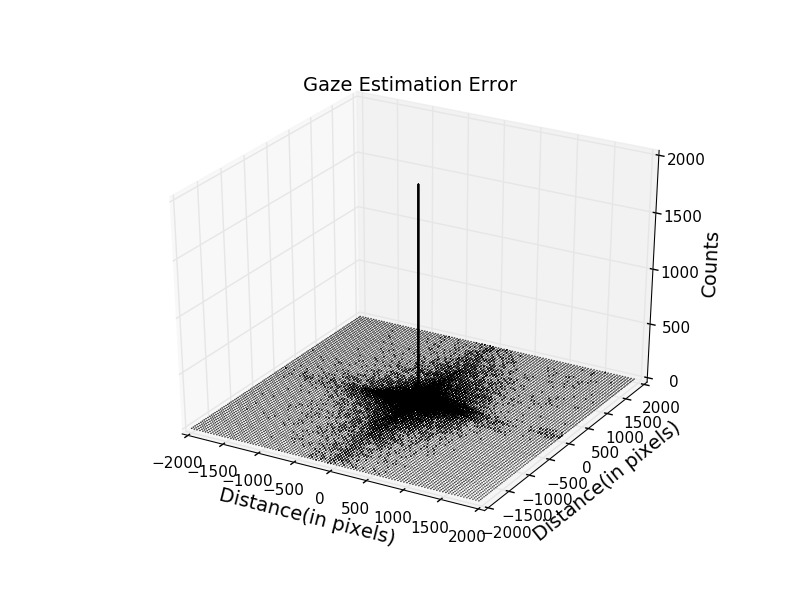
\includegraphics[width=0.5\linewidth,trim={.22\textwidth} {.05\textwidth} {0.12\textwidth} {.05\textwidth},clip]{errorplot1.jpg}
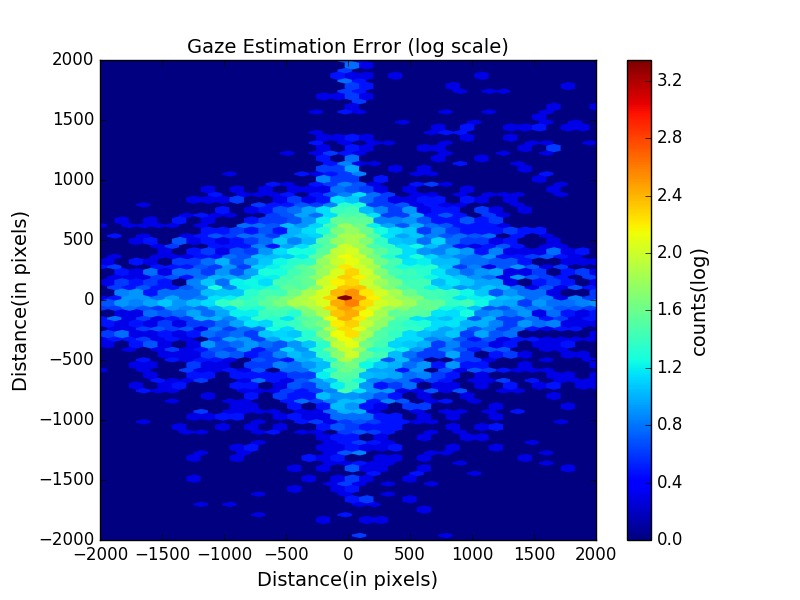
\includegraphics[width=0.5\linewidth,trim={.05\textwidth} {.00\textwidth} {0.132\textwidth} {.05\textwidth},clip]{errorplot.jpg}
%\noindent 
%\noindent
\end{tabular}
\vspace{-1mm}
\caption{Gaze Estimation error distribution. We compute the distance between the gaze estimation coordinates with the groundtruth bounding box along X and Y axis(Centre denotes zero error). Left side figure represents the error in real valued scale and right side in log scale. We choose 2000 pixel distance to match with Cityscapes image dimensions.}
\vspace{-3mm}
\label{fig:gaze_error}
\end{figure}

\subsection{Evaluation}
Out of the $30,000$ annotated objects in our Cityscape dataset~\cite{cityscape}, we use 80\% of videos for the training and 20\% for the evaluation of our model on the task of OR in videos.

\bigskip
\noindent
\textbf{Evaluation Metric}
We evaluate the performance of our language based OR based on Accuracy@1 ($Acc@K$), following ~\cite{hu2016natural,mao2016generation}. 
%$Acc@K$ refers to the percentage of true detections among $K$ top scored object candidates. 
$Acc@1$ refers to the percentage of top scoring candidates being a true detection. A candidate is regarded as a true detection if the Intersection over Union (IoU) computed between the predicted bounding box and ground truth box is more than $0.5$. 
%If the IoU is less than $0.5$, the detection is considered a false positive. 
In all our tables, we compute mean of the $Acc@1$ metric over all the videos in the evaluation set. 


%---------------------------------------------------
\begin{figure}[t!]
\centering
{\tiny \textbf{NLOR}} \hspace{60pt} {\tiny\textbf{Ours: TSCRC}} \hspace{30pt} {\tiny \textbf{Ours: TSCRC+Gaze}}
\begin{tabular}{lll}
\multicolumn{3}{c}{\tiny a woman in front with a white cap is walking towards us on right side of the road along with others}\\
\noindent
\adjustbox{trim={.1\width} {.22\height} {0.1\width} {.22\height},clip}
    {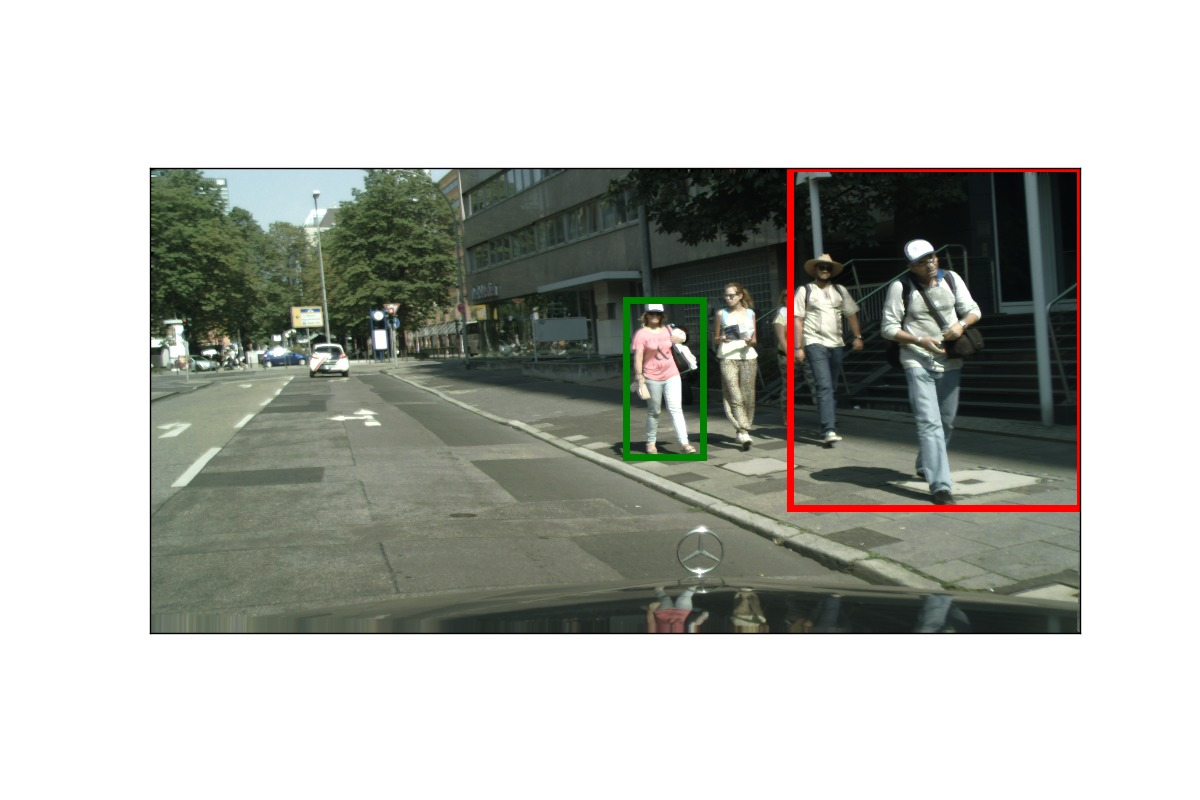
\includegraphics[width=0.4\linewidth]{demo_24_0_nlor.jpg}}
\noindent 
\adjustbox{trim={.1\width} {.22\height} {0.1\width} {.22\height},clip}
    {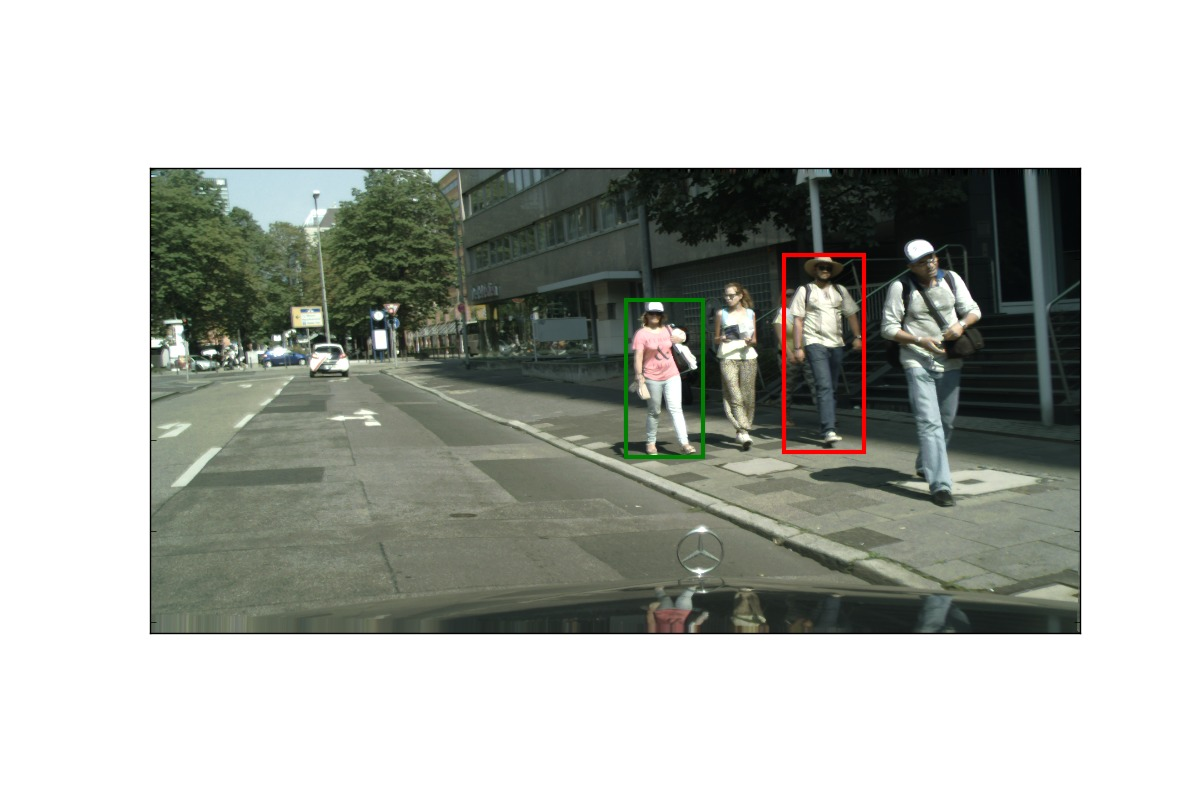
\includegraphics[width=0.4\linewidth]{rdemo_24_0.jpg}}
    \adjustbox{trim={.1\width} {.22\height} {0.1\width} {.22\height},clip}
    {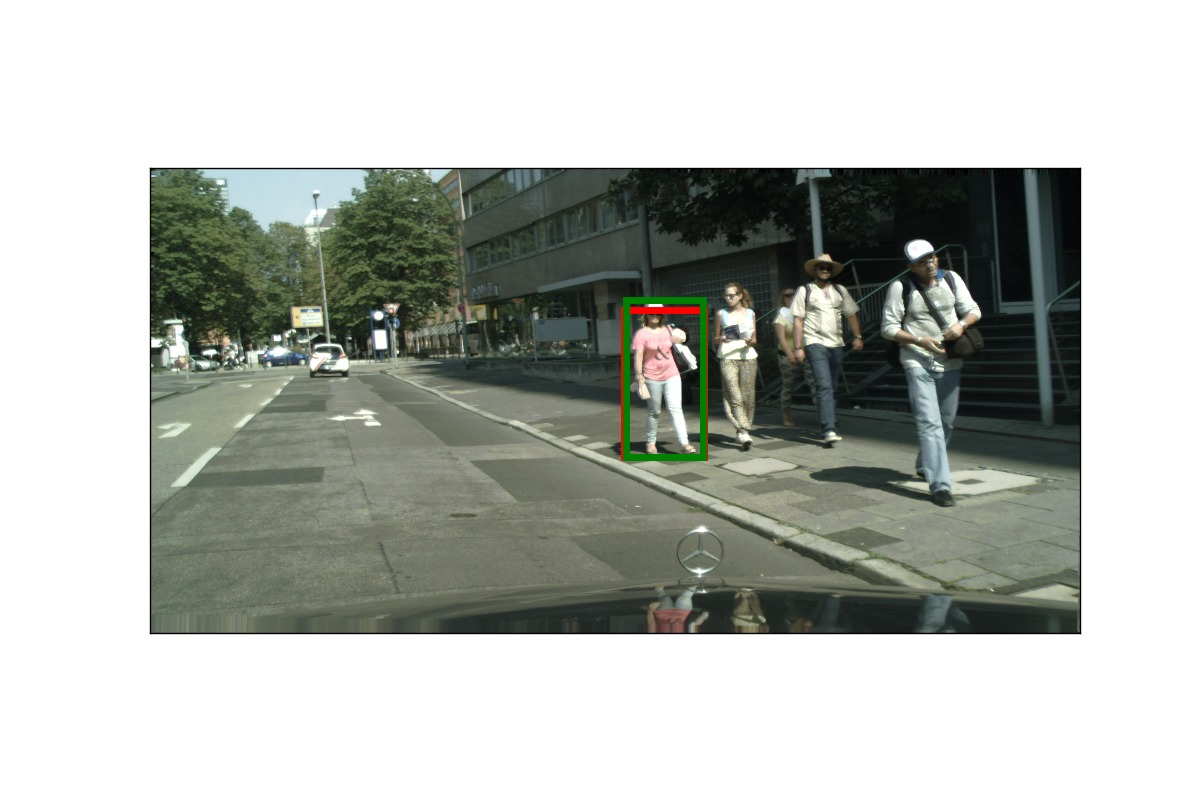
\includegraphics[width=0.4\linewidth]{demo_24_0.jpg}} \vspace{-1mm}\\
    \multicolumn{3}{c}{\tiny a huge car is turning right side of the road near the building area}\\
   % \vspace{0.02cm}
    \adjustbox{trim={.1\width} {.22\height} {0.1\width} {.24\height},clip}
    {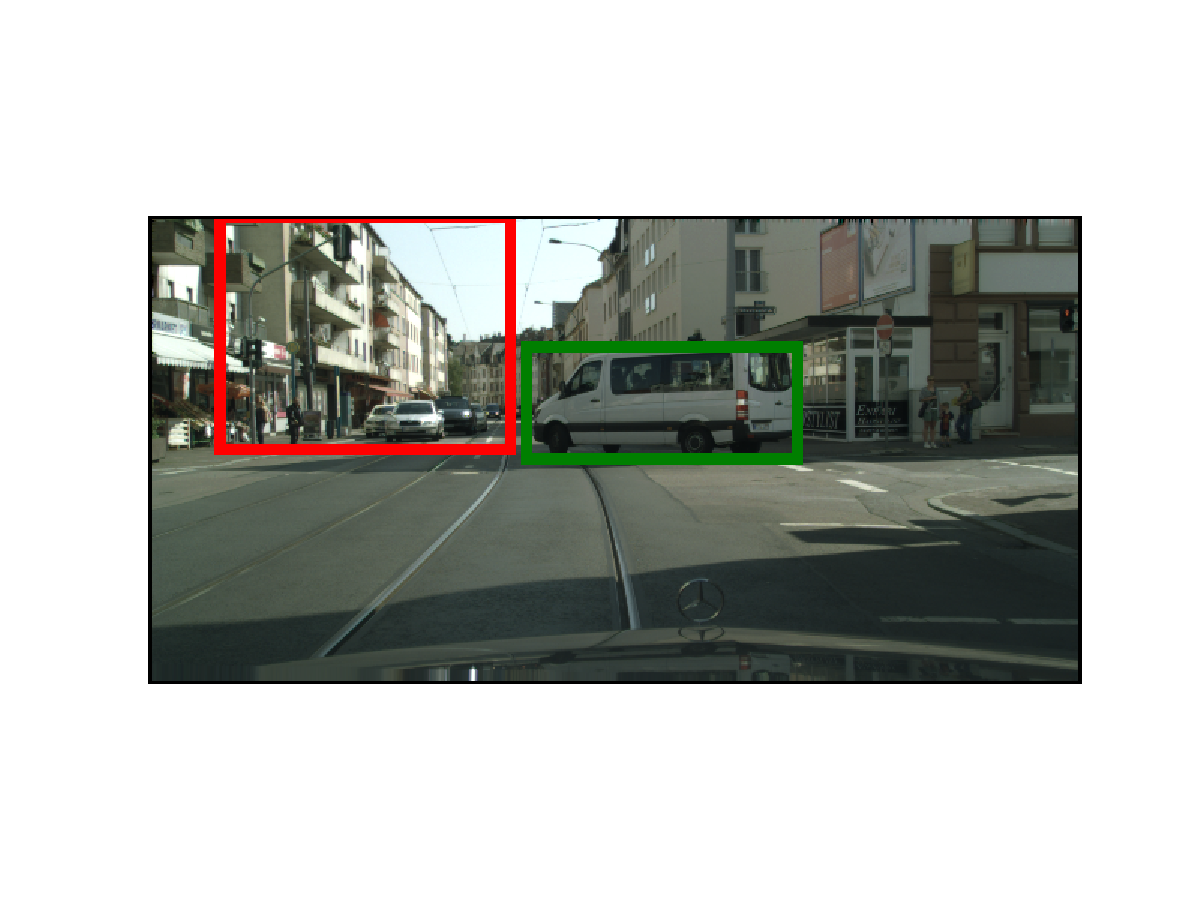
\includegraphics[width=0.4\linewidth]{demo_5_0_nlor.pdf}}
\noindent 
\adjustbox{trim={.1\width} {.22\height} {0.1\width} {.24\height},clip}
    {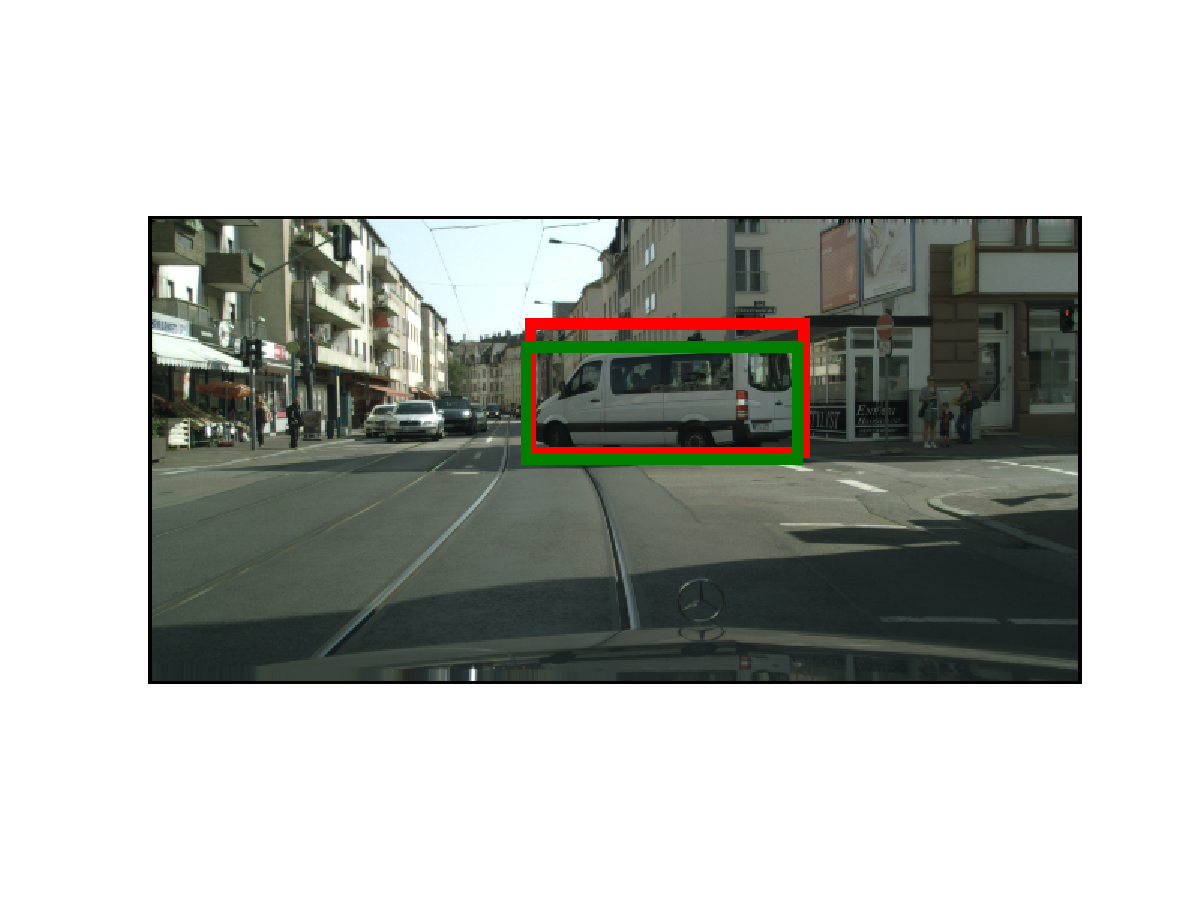
\includegraphics[width=0.4\linewidth]{demo_5_0_mm.pdf}}
    \adjustbox{trim={.1\width} {.18\height} {0.1\width} {.20\height},clip}
    {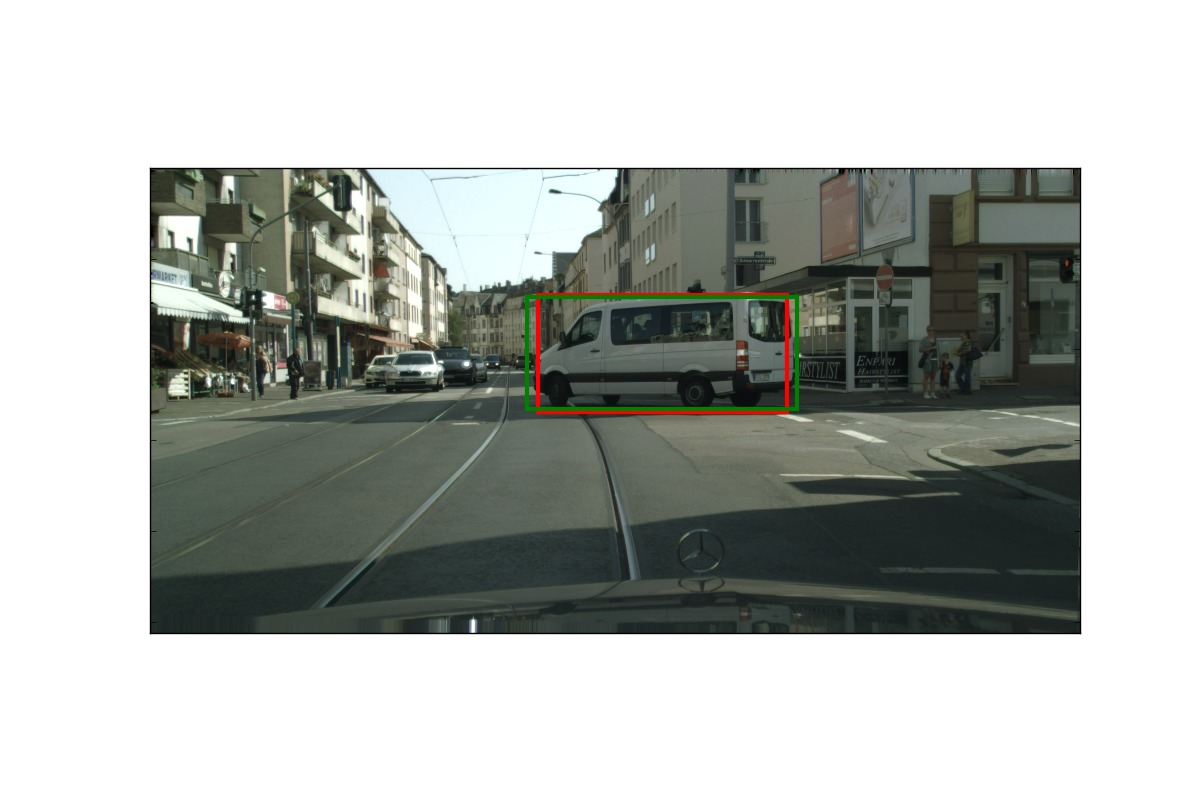
\includegraphics[width=0.4\linewidth]{rdemo_5_0.jpg}} \vspace{-1mm} \\
    \multicolumn{3}{c}{\tiny a woman in white dress in front is walking towards us on right side of road along with her family.}\\
        \adjustbox{trim={.1\width} {.2\height} {0.1\width} {.22\height},clip}
    {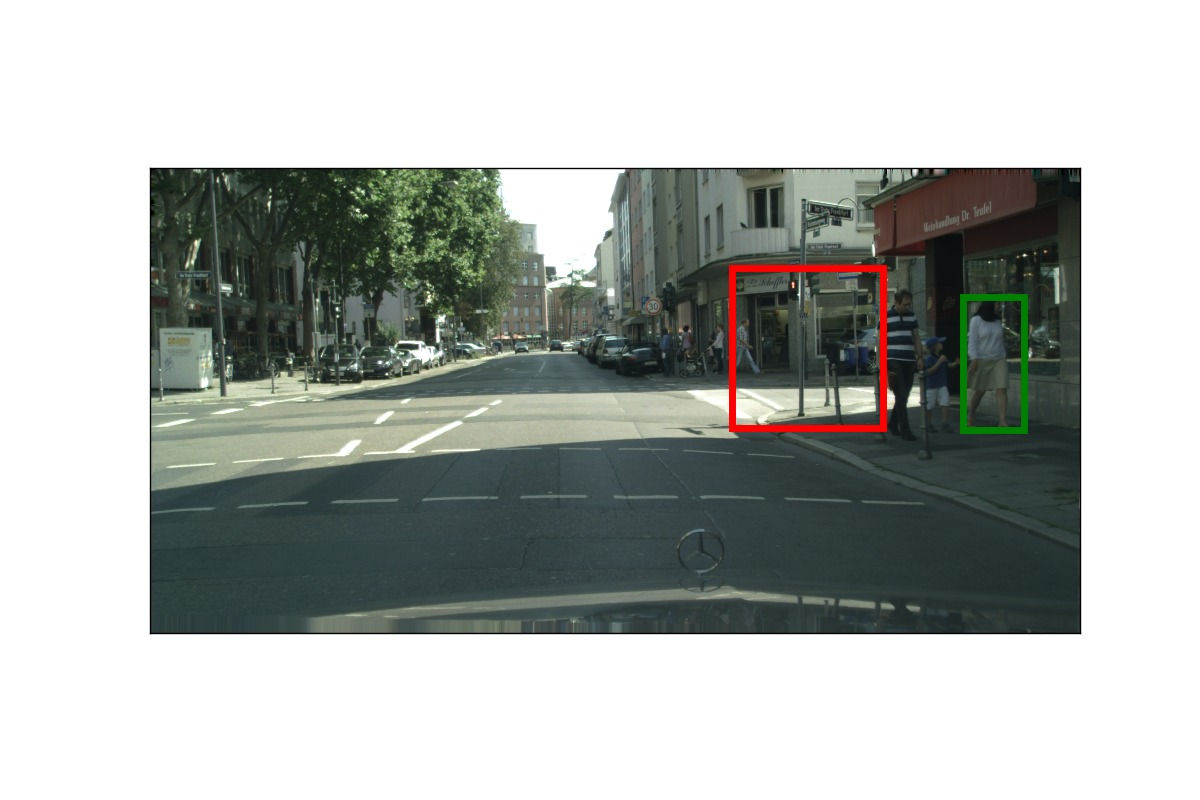
\includegraphics[width=0.4\linewidth]{demo_44_0_nlor.jpg}}
\noindent 
\adjustbox{trim={.1\width} {.2\height} {0.1\width} {.22\height},clip}
          {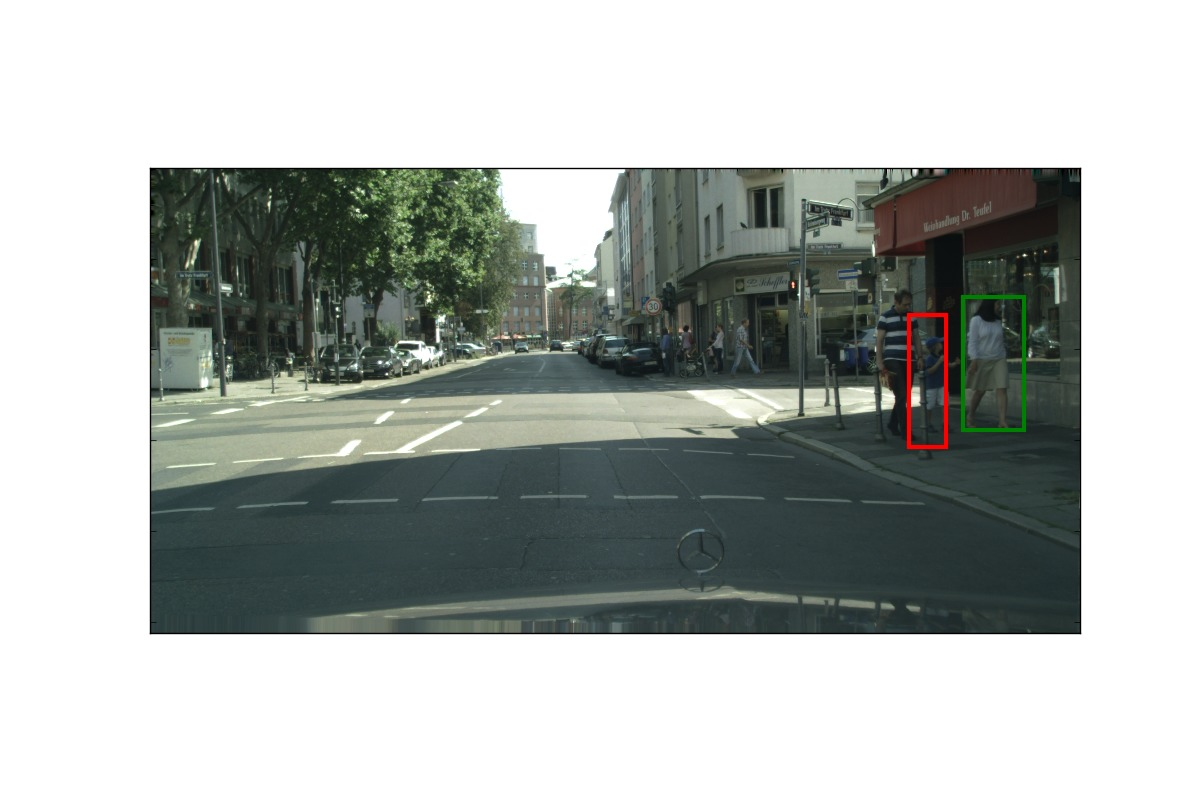
\includegraphics[width=0.4\linewidth]{rdemo_44_0.jpg}}
    \adjustbox{trim={.1\width} {.2\height} {0.1\width} {.22\height},clip}
    {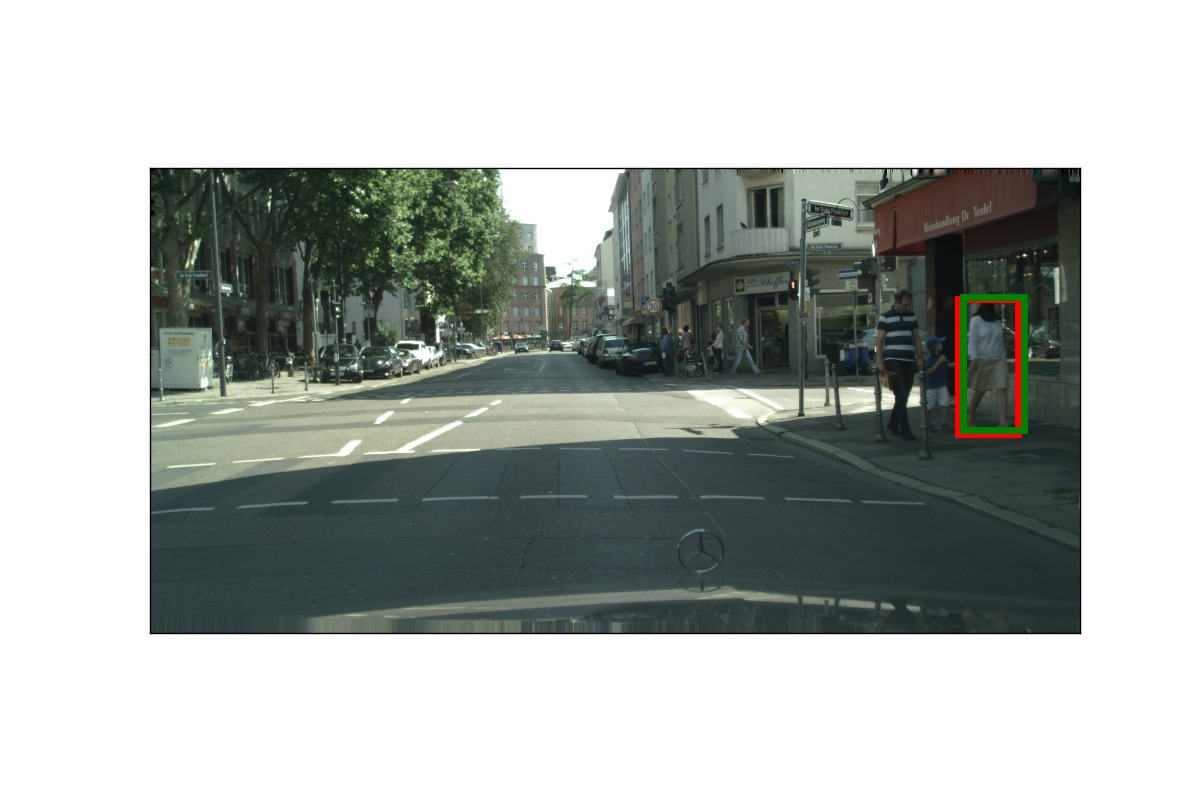
\includegraphics[width=0.4\linewidth]{demo_44_0.jpg}} \vspace{-1mm}\\ 
    \multicolumn{3}{c}{\tiny a car in front at a very far distance is moving on left side of the road}\\
            \adjustbox{trim={.1\width} {.2\height} {0.1\width} {.22\height},clip}
    {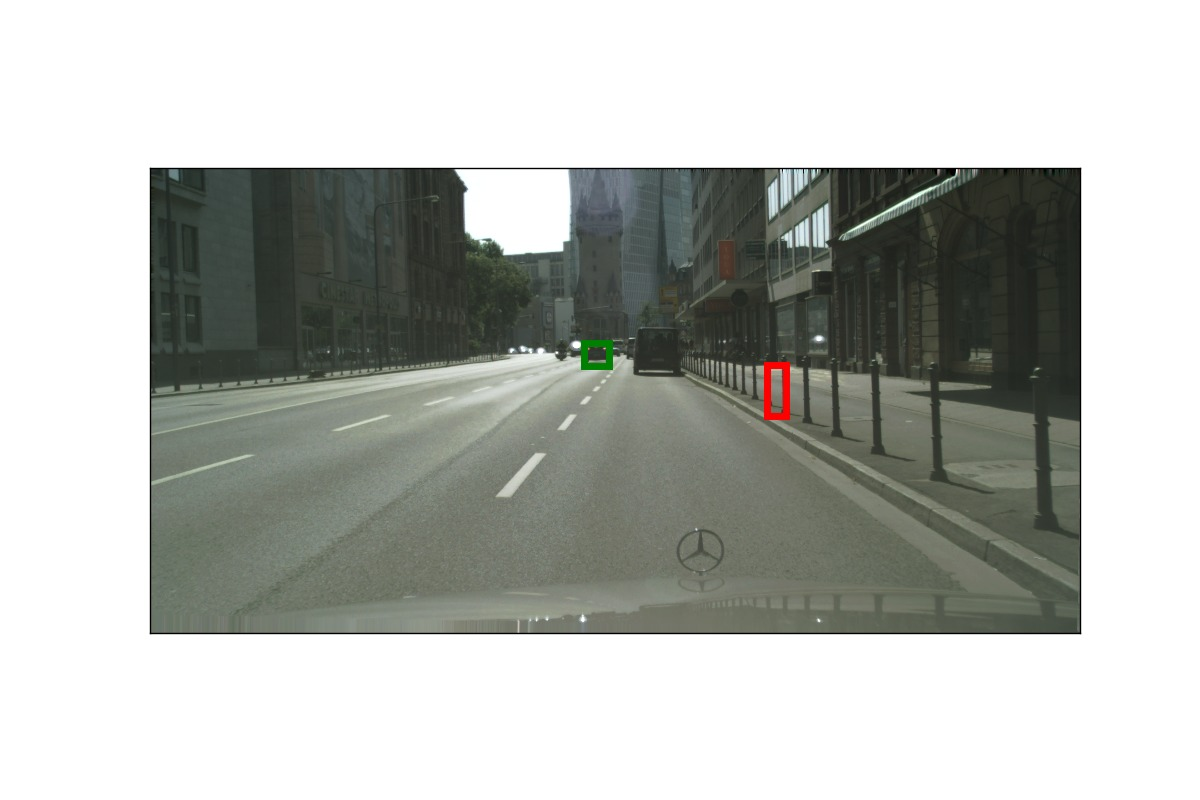
\includegraphics[width=0.4\linewidth]{demo_46_0_nlor.jpg}}
\noindent 
\adjustbox{trim={.1\width} {.2\height} {0.1\width} {.22\height},clip}
    {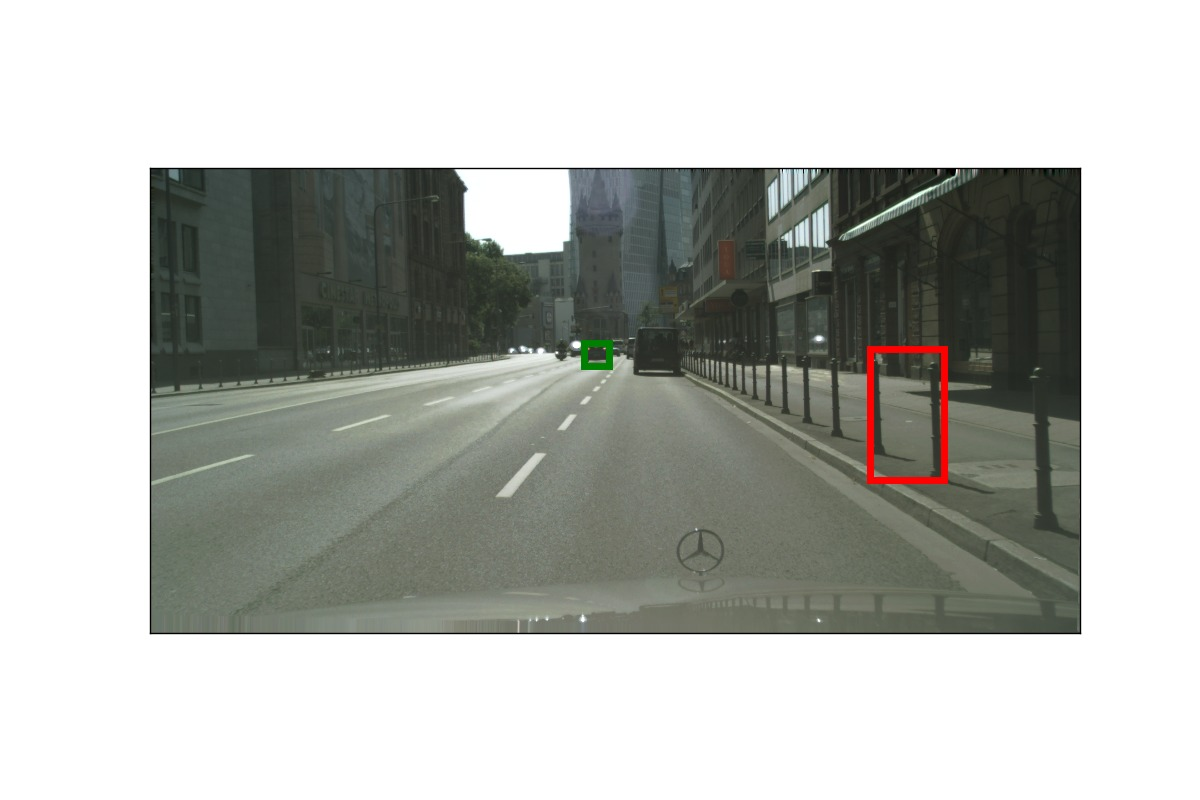
\includegraphics[width=0.4\linewidth]{demo_46_0_mm.jpg}}
    \adjustbox{trim={.1\width} {.2\height} {0.1\width} {.22\height},clip}
    {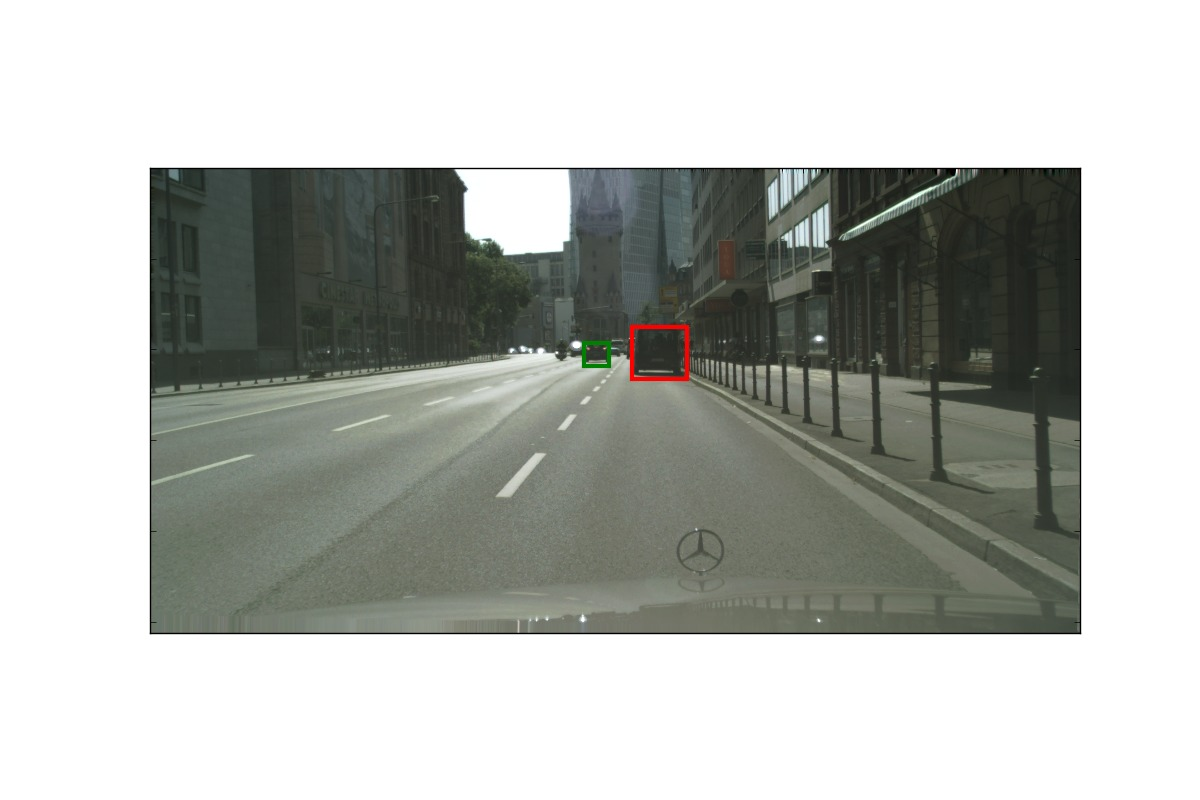
\includegraphics[width=0.4\linewidth]{rdemo_46_0.jpg}}\\
%\noindent 
%\includegraphics[width=0.5\linewidth]{Recall-IoU-100proposals.jpg}
%\noindent 
%\includegraphics[width=0.5\linewidth]{Recall-Candidates-IoU_0_9.jpg}
\end{tabular}
\caption{Some qualitative results from: NLOR (left column), Ours(I,D,O) (middle) and Ours(I,D,O,G) (right column). These results are obtained on the Cityscapes.  {\color{green} Green}: ground truth box and {\color{red}Red}: predicted box.}
\label{fig:qual-results-cityscape}
\vspace{-1mm}
\end{figure}
%---------------------------------------------------


%-----------------------------------------------------
\begin{figure*} 
  \centering
   $ \begin{array}{cccccc}  \hspace{-4mm}
 \begin{turn}{90}{\scriptsize{Descriptions}}\end{turn} & \hspace{-3mm}
\begin{tcolorbox}[width=0.24\linewidth, left=1pt,right=1pt,top=0pt,bottom=0pt]
a woman in front is crossing the road from left to right side with a travel bag
\end{tcolorbox} 
& \hspace{-2mm}
\begin{tcolorbox}[width=0.24\linewidth, left=1pt,right=1pt,top=0pt,bottom=0pt]
a red car in front is parked on right side of road along with other cars             
\end{tcolorbox} 
& \hspace{-2mm}
\begin{tcolorbox}[width=0.24\linewidth, left=1pt,right=1pt,top=0pt,bottom=0pt]
a woman in front is crossing the road from right to left with others
\end{tcolorbox} 
& \hspace{-2mm}
\begin{tcolorbox}[width=0.24\linewidth, left=1pt,right=1pt,top=0pt,bottom=0pt]
a man in front is walking on the left side of another road
\end{tcolorbox} \vspace{-4.5mm} \\ \hspace{-4mm}
 \begin{turn}{90}{\scriptsize{Video and Gaze}}\end{turn}
\hspace{0.6mm} & \hspace{-3mm}
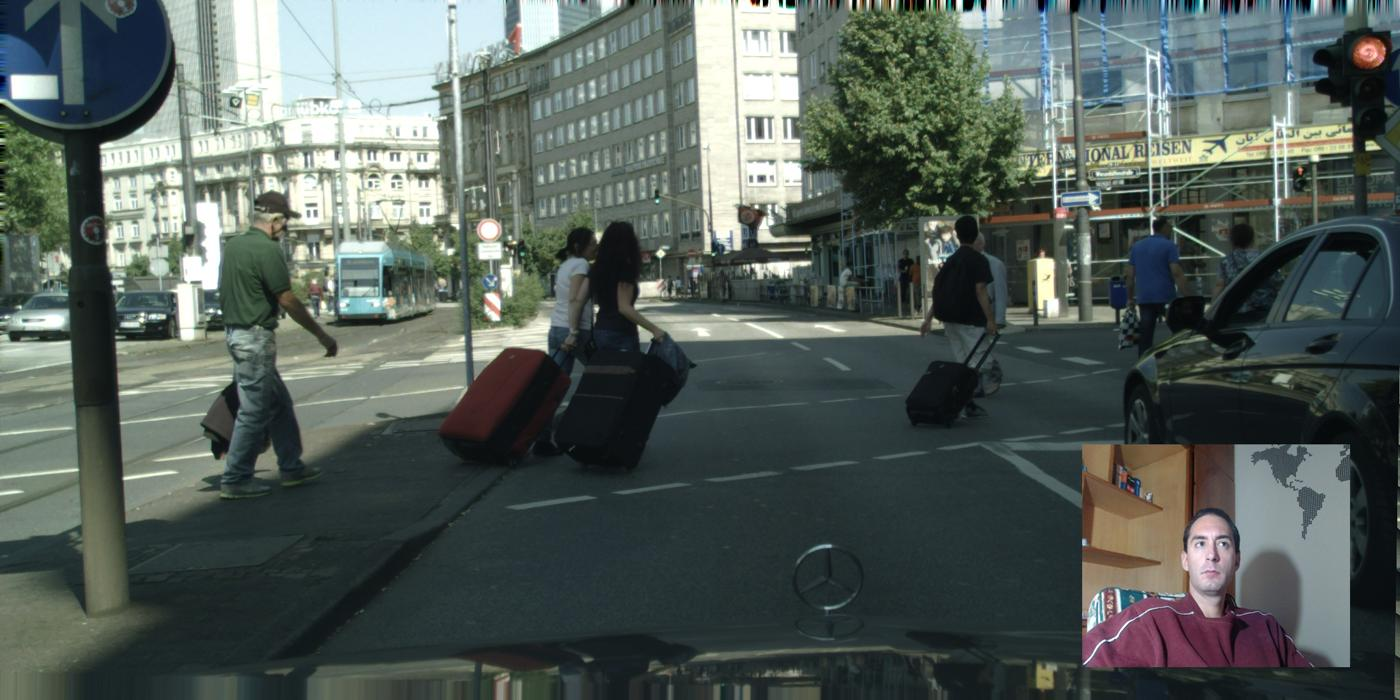
\includegraphics[width=0.24\linewidth]{frankfurt_000140_000029_leftImg8bit_modf.jpg} & 
    \hspace{-2mm}
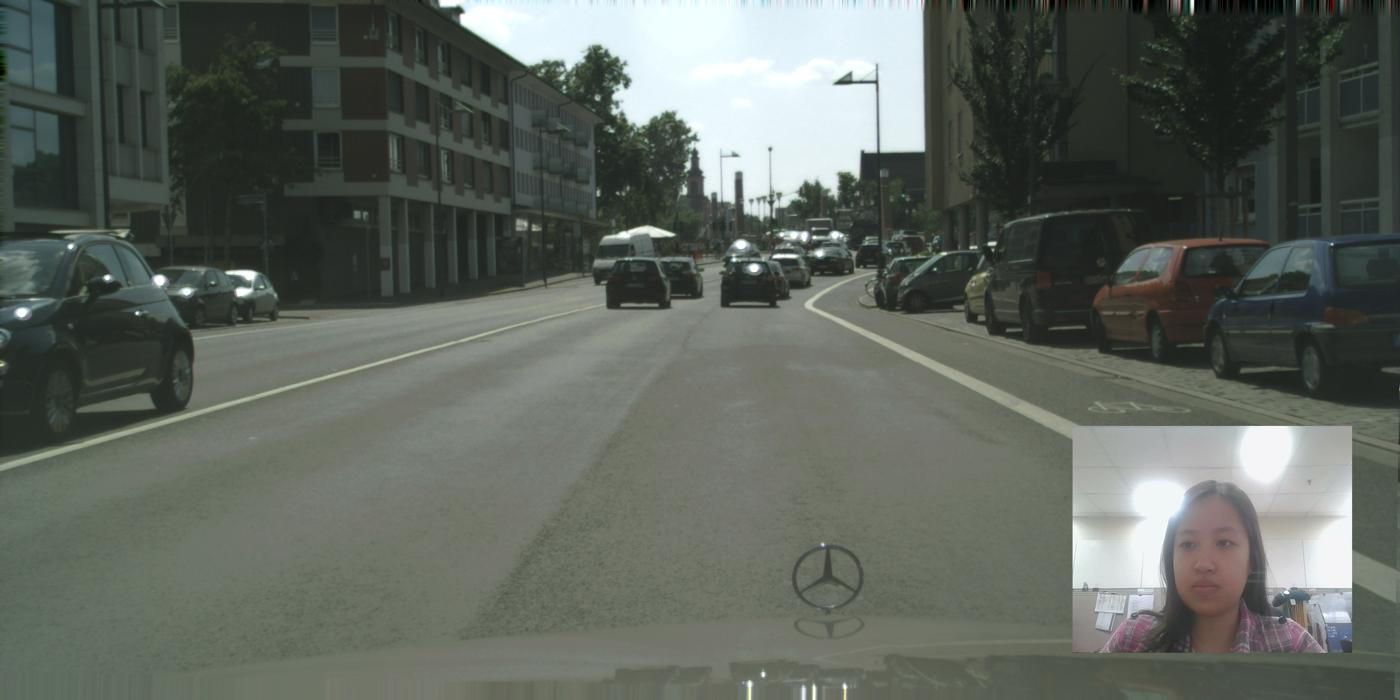
\includegraphics[width=0.24\linewidth]{frankfurt_000208_000029_leftImg8bit_modf.jpg} &  
    \hspace{-2mm}
 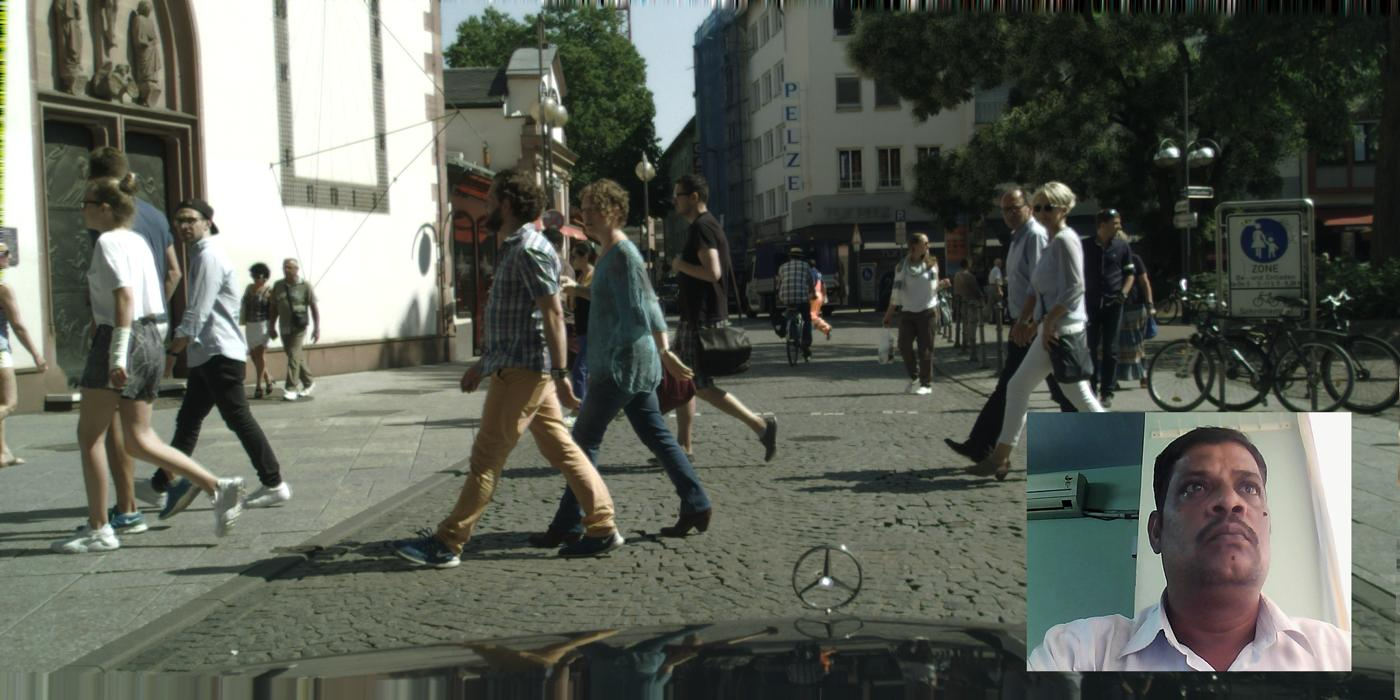
\includegraphics[width=0.24\linewidth]{frankfurt_000080_000029_leftImg8bit_modf.jpg} & 
    \hspace{-2mm}
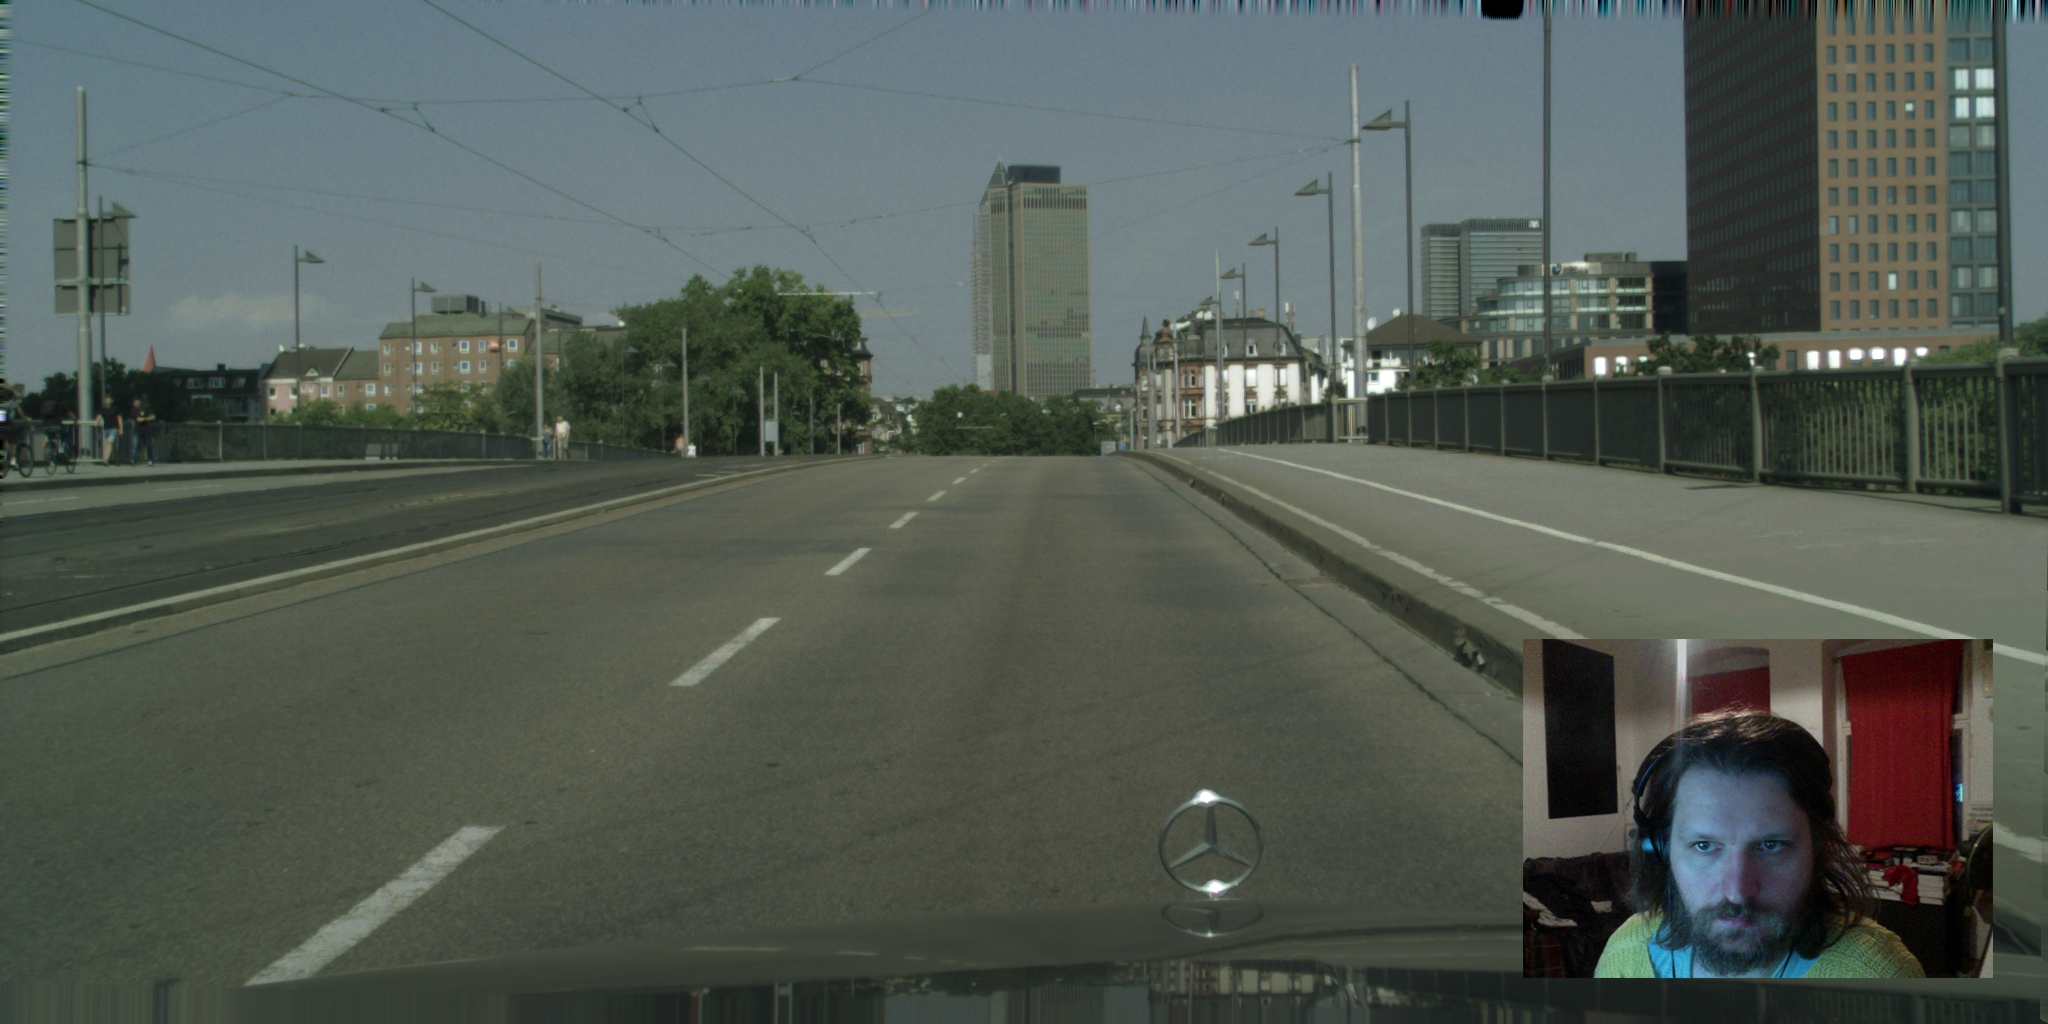
\includegraphics[width=0.24\linewidth]{frankfurt_000019_000029_leftImg8bit_modf.jpg} \vspace{1.5mm} \\ \hspace{-4mm}

 \begin{turn}{90}{\scriptsize{Intermediate Results}}\end{turn}
 \hspace{0.6mm}
&  \hspace{-3mm}
     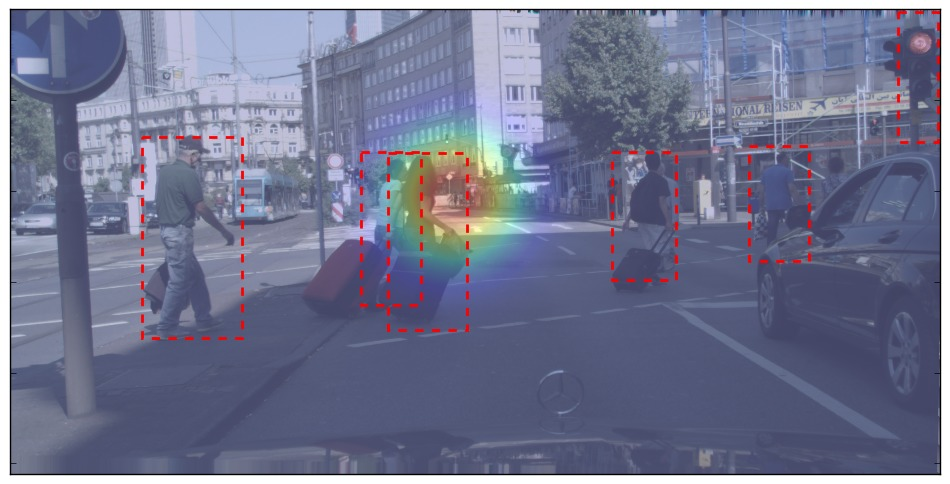
\includegraphics[width=0.24\linewidth]{demo_140_0.jpg}
 
& \hspace{-2mm}
     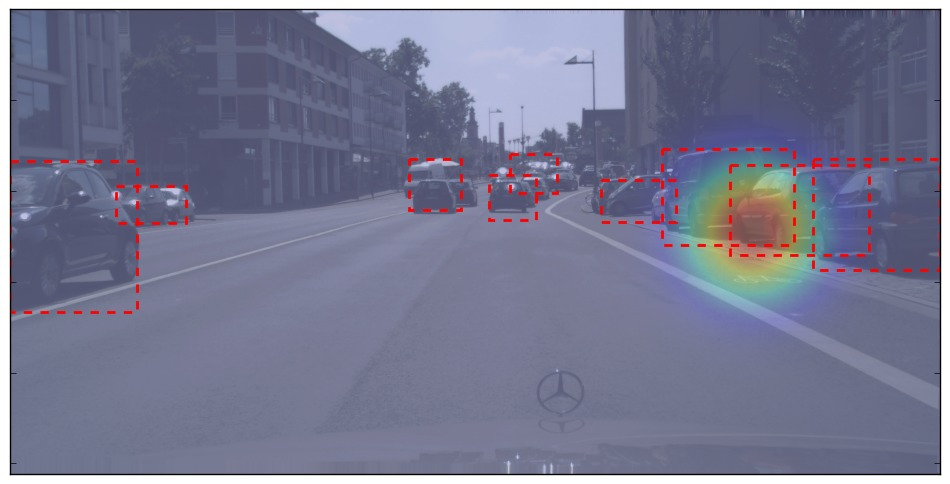
\includegraphics[width=0.24\linewidth]{demo_208_0.jpg}

& \hspace{-2mm}
     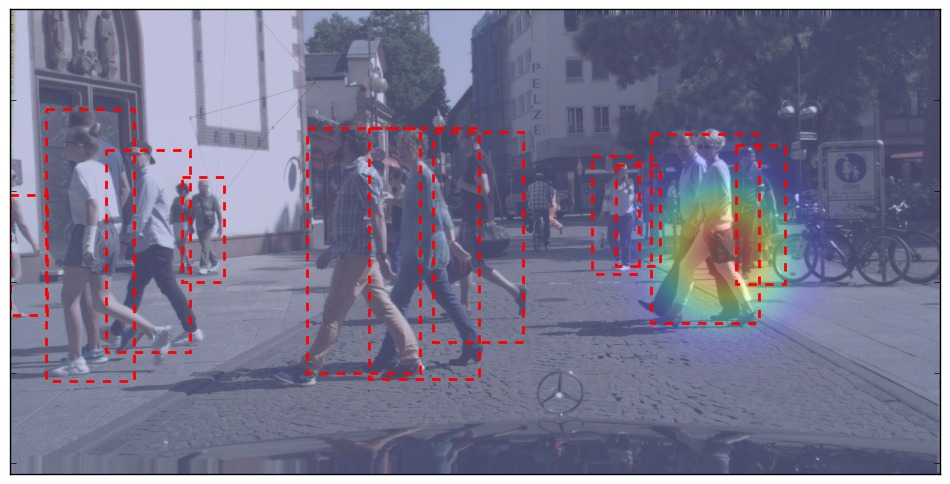
\includegraphics[width=0.24\linewidth]{demo_80_0.jpg}
    
& \hspace{-2mm}
    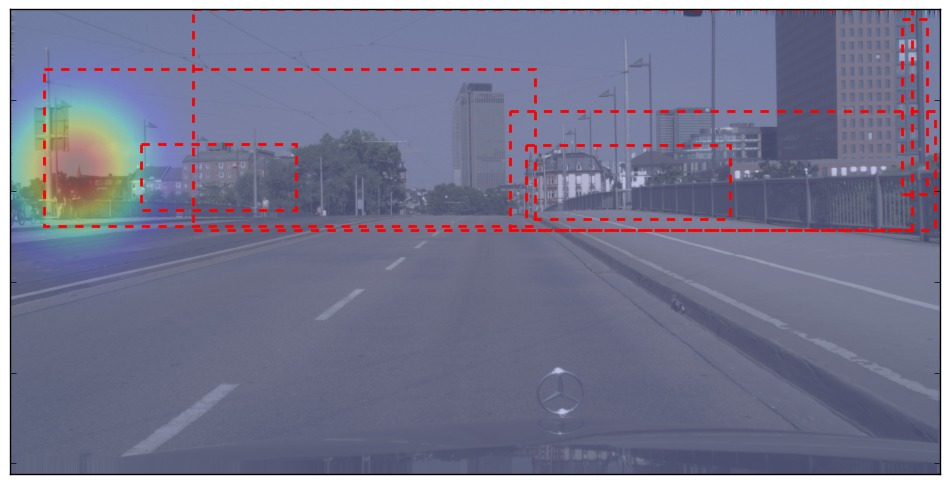
\includegraphics[width=0.24\linewidth]{demo_19_0.jpg} \vspace{1.2mm}
\\ \hspace{-3mm}
 \begin{turn}{90}{\scriptsize{Final Results}}\end{turn}
 \hspace{0.6mm}  
& \hspace{-3mm} 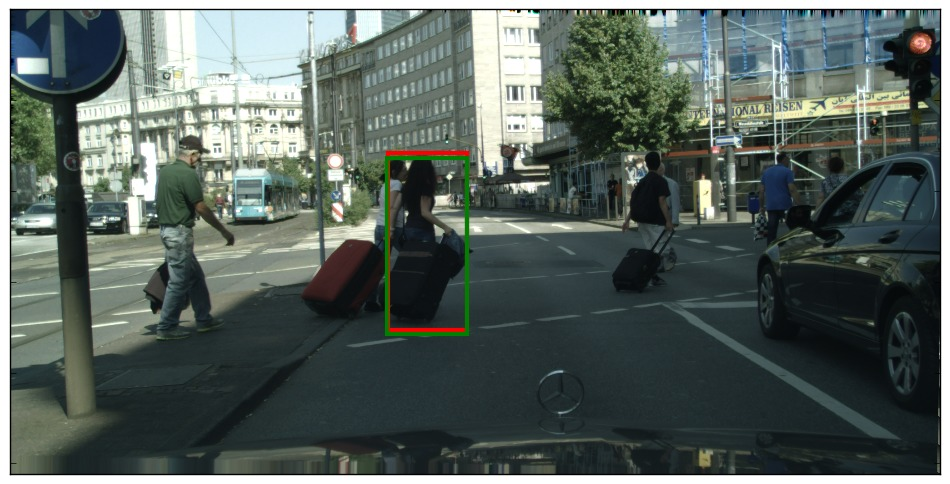
\includegraphics[width=0.24\linewidth]{rdemo_140_0.jpg}

& \hspace{-2mm} 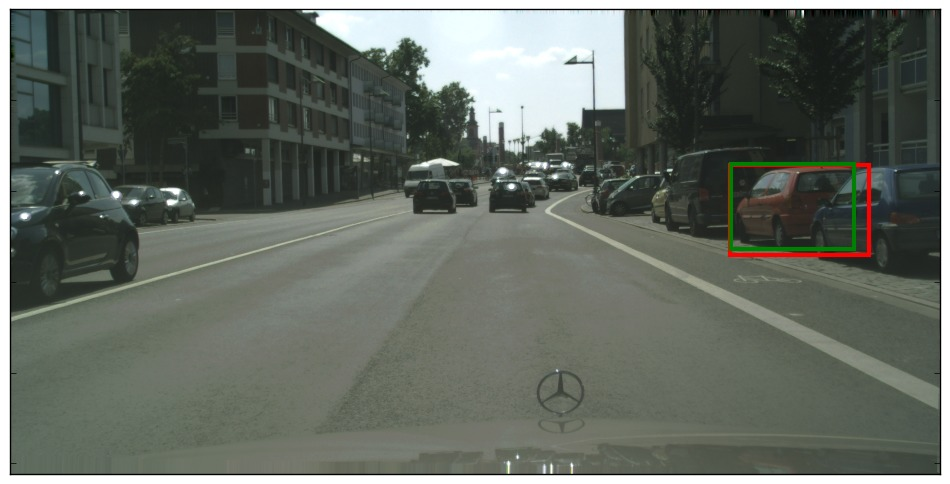
\includegraphics[width=0.24\linewidth]{rdemo_208_0.jpg}

& \hspace{-2mm} 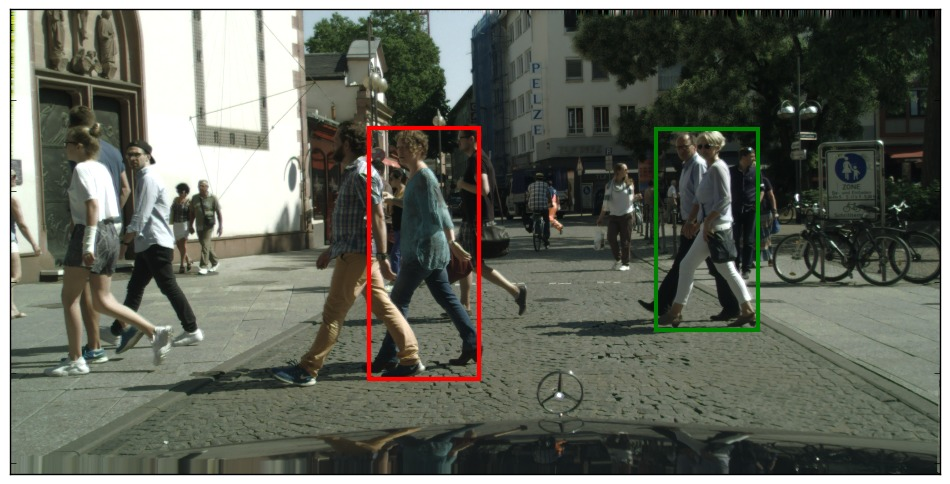
\includegraphics[width=0.24\linewidth]{rdemo_80_0.jpg}

& \hspace{-2mm} 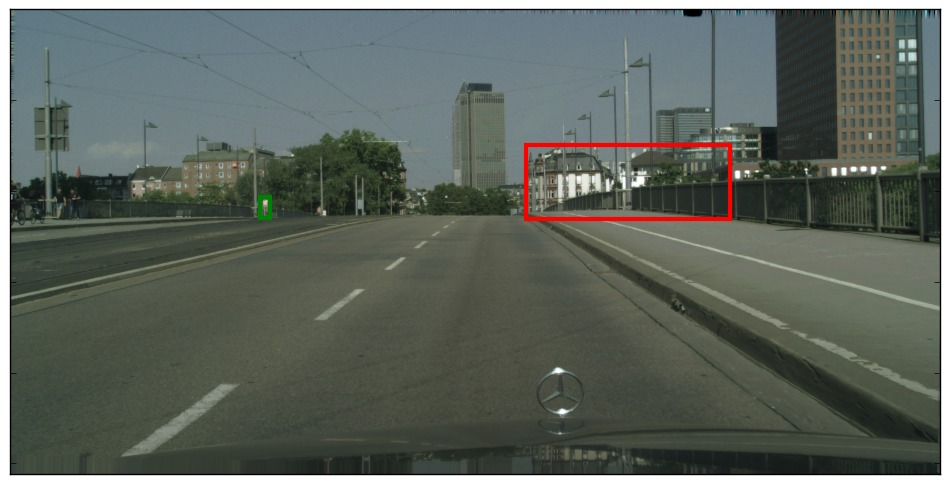
\includegraphics[width=0.24\linewidth]{rdemo_19_0.jpg}
\\
\end{array}$
\caption{Overall results on Cityscapes. Input descriptions on the first row and input videoframe and gaze in the second row. Middle row represents intermediate results where Gaze estimation is embedded along with object proposals while bottom row represents the final OR results. {\color{green} Green}: ground truth box and {\color{red}Red}: proposals and the predicted boxes.}
\label{fig:qual-gaze-results-cityscape}
\end{figure*}
%-----------------------------------------------

\bigskip
\noindent
\textbf{Object Proposal}
We use object proposal techniques such as Edgebox~\cite{ZitnickECCV14edgeBoxes}, FRCNN~\cite{renNIPS15fasterrcnn} and LOP~\cite{vasudevan2017chi} and we have tabulated the comparison between them in Tab.~\ref{tab:eop-expt}. Since LOP performs consistently better for OR, we use the same for all the later experiments.
%LOP has two sub-networks: FRCNN and LSTM. We train FRCNN for the object detection task on $20$ object classes of the Cityscape dataset. We use the segmentation annotation of the Cityscape training set to generate bounding boxes for objects. We use the pre-trained weights for FRCNN trained on Pascal VOC to leverage the overlap of object classes in Cityscape and Pascal VOC. We train an LSTM network using all the referring expressions which we annotated as part of the Cityscape training set. The network achieves a validation accuracy of $91.5$\%. 

%In Table~\ref{tab:cityscape}, we again evaluate the improvement by our proposal method to language-based object detection (LOD) with different modalities, from only RGB images, through RGB + depth and RGB + motion, to the combination of all three. From the table, we can see  an improvement of $14.64$\% in $Acc@1$ for $30$ object proposals comparing Ours:Img-HHA-Flow+FRCNN and Ours:Img-HHA-Flow+LOP which indicates the effectiveness of LOP for the task of LOD across different combinations of data modalities.

\bigskip
\noindent
\textbf{Images vs. Stereo Videos}.
The performance of our model using different modalities and their combinations is reported in Tab.~\ref{tab:eop-expt}. From the table, we can see that our model can effectively utilize the additional modalities such as depth and motion provided in stereo videos.  
For instance, the $Acc@1$ is improved by $6.242$\% by using depth and motion; that is the improvement of Ours (I,D,O) over NLOR under LOP for 30 object proposals(I:RGB, D:Depth map, O:Optical Flow, G:Gaze). 
%Ours (I,D,O) and $9.17$\% from NLOR to Ours(I,D,O,G)  
We observe similar improvement For FRCNN as object proposals. Since LOP is consistent over all methods, we choose LOP as proposal technique for Tab.~\ref{tab:cityscape-track} and Tab.~\ref{tab:gaze-comparison}. We observe that both depth and motion can enhance the performance of OR, on top of RGB appearances alone. For example, depth improves the performance by $4.053$\% and motion improves it by $5.360$\%. The combination of all the three: appearance, depth, and motion, yields the best results. This indicates that spacial information and motion are very useful for the task of Object Referring. This is due to the fact that human do use these features to describe objects as mentioned in the Sec.\ref{sec:intro}. Please see Fig.~\ref{fig:qual-results-cityscape} for some visual results and how the three additional modalities (D,O,G) improve the detections over the original work of~\cite{hu2016natural}. 

%from Ours(I) while $G$ by $1.928$\% from Ours(I,D,O).
%Our main focus is on the $Acc@1$ metric as a top-1 accuracy is more significant for the object detection task. 
%We did not see the corresponding improvement at $Acc@10$ and at higher number of object proposals. This is because when we allow high number of proposals, the number of poor candidates also get increased which confuses TSCRC model and yield many false positives.

It is also observed from the table that motion feature is more useful than depth information or it is just better utilized by our model. This can be ascribed to the fact that the convolutional network to extract motion features was trained with a much large dataset than that for the network of depth features. A better representation of depth than HHA images can be a good research topic for further improvement. 
%Also, extending the model to longer temporal context is part of our future work. 
In Tab.~\ref{tab:cityscape-track}, we included flow information from the past by experimenting on different track length. We see that longer tracks do not bring significant improvement to OR accuracy. This may be because a) the referring expressions are annotated for the last frame and b) the length of Cityscapes's videos are just 2 seconds long to bring any significant change in motion. 
%Nevertheless, the model learns useful information from motion and depth already. 

%The combination of TSCRC and LOP outperforms the original approach of Hu \etal~\cite{hu2016natural} for $Acc@1$ by a large margin. %The main advantage of the combination is that LOP gives a variable number of object proposals specific to the sample depending on the referring expression and FRCNN detections. This, in a way, ensures that not many poor candidates are passed to the TSCRC model.

%\bigskip
%\noindent
%\textbf{Gaze Estimation}
\bigskip
\noindent
\textbf{Gaze vs. w/o Gaze}.
Gaze features are given to our model as additional local features along with depth and flow features. Comparing our model with and without Gaze, we observe that Gaze improves the performance of our model significantly for all the variants of our model as in Tab.~\ref{tab:gaze-comparison}. For instance Gaze features under Max pooling improve the performance by $2.809$\% for image-only case (Ours (I)); by $1.993$\% for the case where image and motion are used (Ours (I,O)); and by $1.928$\% when image, motion and depth are all used (Ours (I,D,O)). The experimental results show that human gaze consistently improves the performance for object referring. This is due to the fact that human do gaze at object when issuing referring expressions. 

Since there arises sampling rate difference between Cityscape video and gaze recording video, we experimented on extracting gaze features under two cases: a) timestamp matching between the videos, b) \# gaze frames $>$ \# frames in Cityscapes video, where we tried average pooling and max pooling of object features to ensure one-to-one correspondence between frames of the two videos. From Tab.~\ref{tab:gaze-comparison}, we observe that max pooling of object features performs as good or better than other cases such as averaging pooling. Because, errors due to quick change of eye gaze(outliers) can be avoided by max-pooling the object features.

% {\tiny \textbf{a woman in front is crossing the road from left to right side with a travel bag in hand}} \hspace{1pt} {\tiny\textbf{a red car in front is parked on right side of road along with other cars}} \hspace{1pt} {\tiny \textbf{a woman in front is crossing the road from right to left with others}\hspace{1pt} {\tiny \textbf{a man in front is walking on left side of another road}}}

% \begin{figure*}[t]
% \centering
% {\tiny \textbf{a woman in front is crossing the road from left to right side with a travel bag in hand}} \hspace{1pt} {\tiny\textbf{a red car in front is parked on right side of road along with other cars}} \hspace{1pt} {\tiny \textbf{a woman in front is crossing the road from right to left with others}\hspace{1pt} {\tiny \textbf{a man in front is walking on left side of another road}}}

% \begin{tabular}{cccccc}
% %\multicolumn{3}{c}{\tiny a black color car in front is turning to its right from right side of road}\\
% %\noindent
% \begin{turn}{90}{\scriptsize Raw Inputs}\end{turn}%\begin{turn}{90}{\scriptsize dangerous}\end{turn}
% \hspace{0.2cm}
%  &
%  \adjustbox{trim={.01\width} {.02\height} {0.01\width} {.02\height},clip}
%     {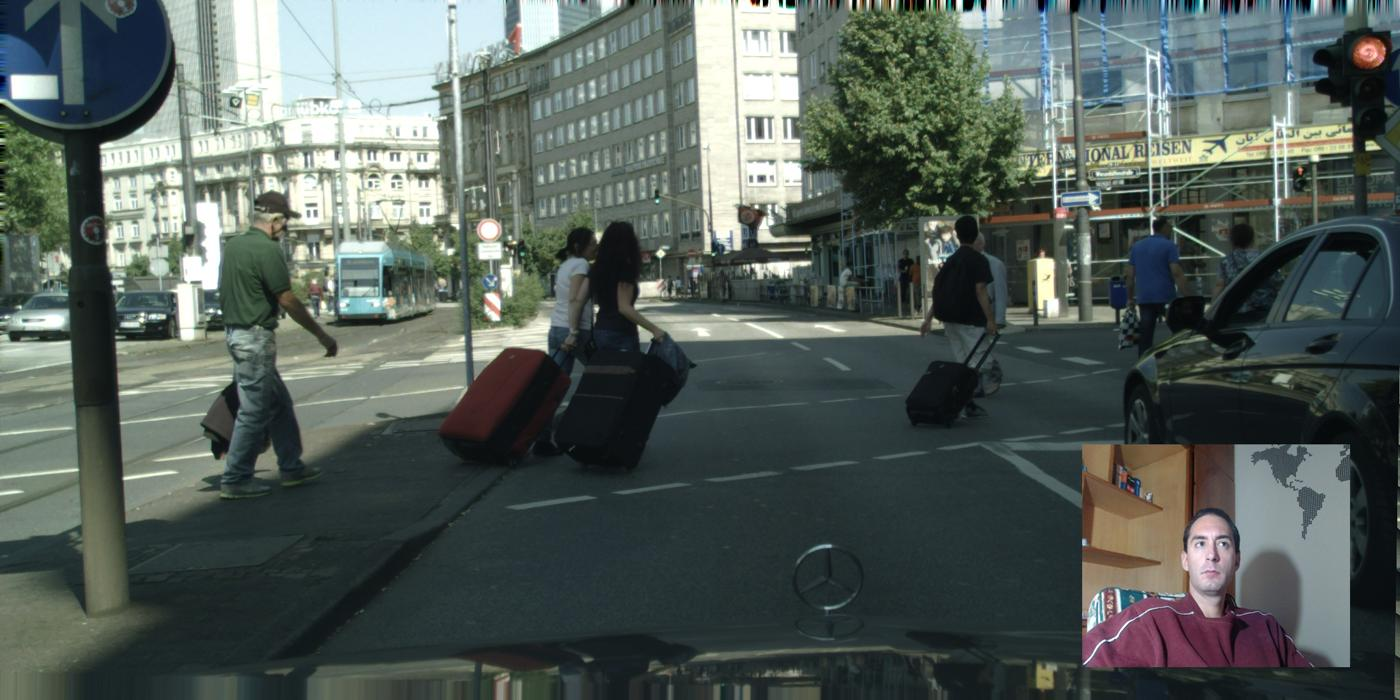
\includegraphics[width=0.23\linewidth]{frankfurt_000140_000029_leftImg8bit_modf.jpg}}
% \hspace{0.2cm} 
% &
%  \adjustbox{trim={.01\width} {.02\height} {0.01\width} {.02\height},clip}
%     {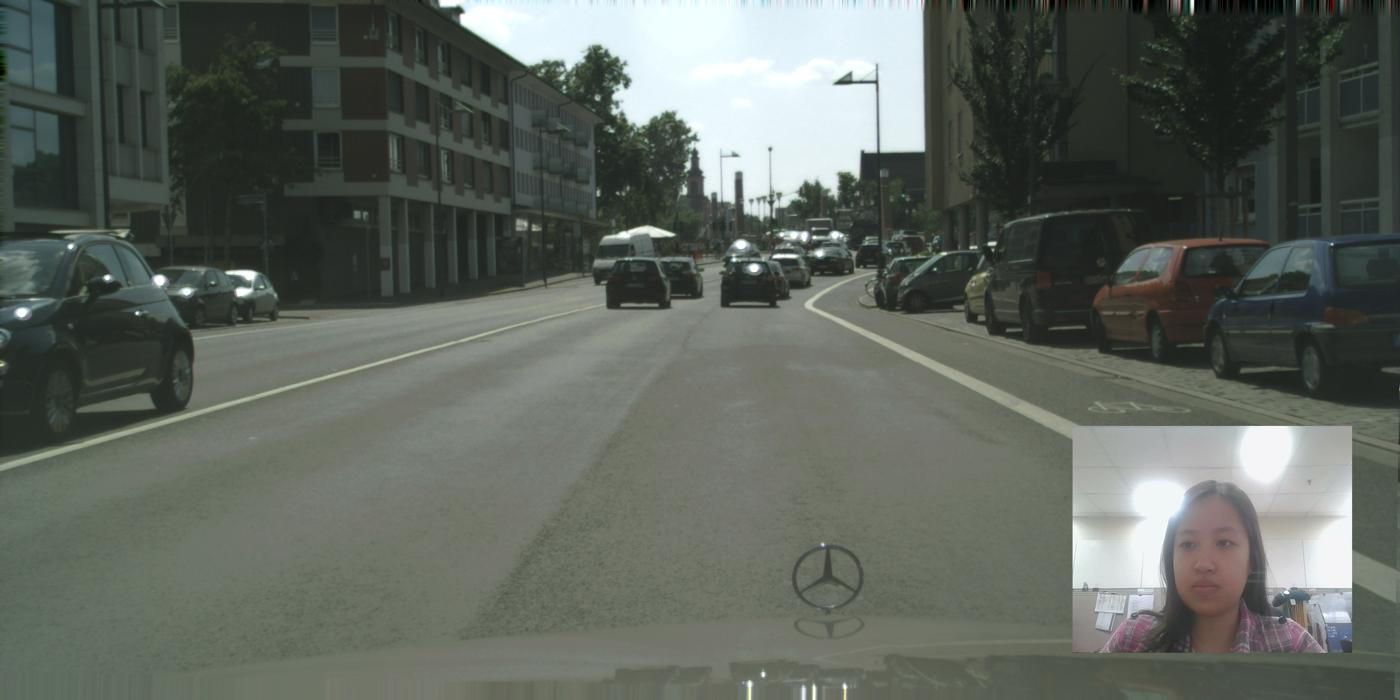
\includegraphics[width=0.23\linewidth]{frankfurt_000208_000029_leftImg8bit_modf.jpg}}
% \hspace{0.2cm}
% &
%             \adjustbox{trim={.01\width} {.02\height} {0.01\width} {.02\height},clip}
%     {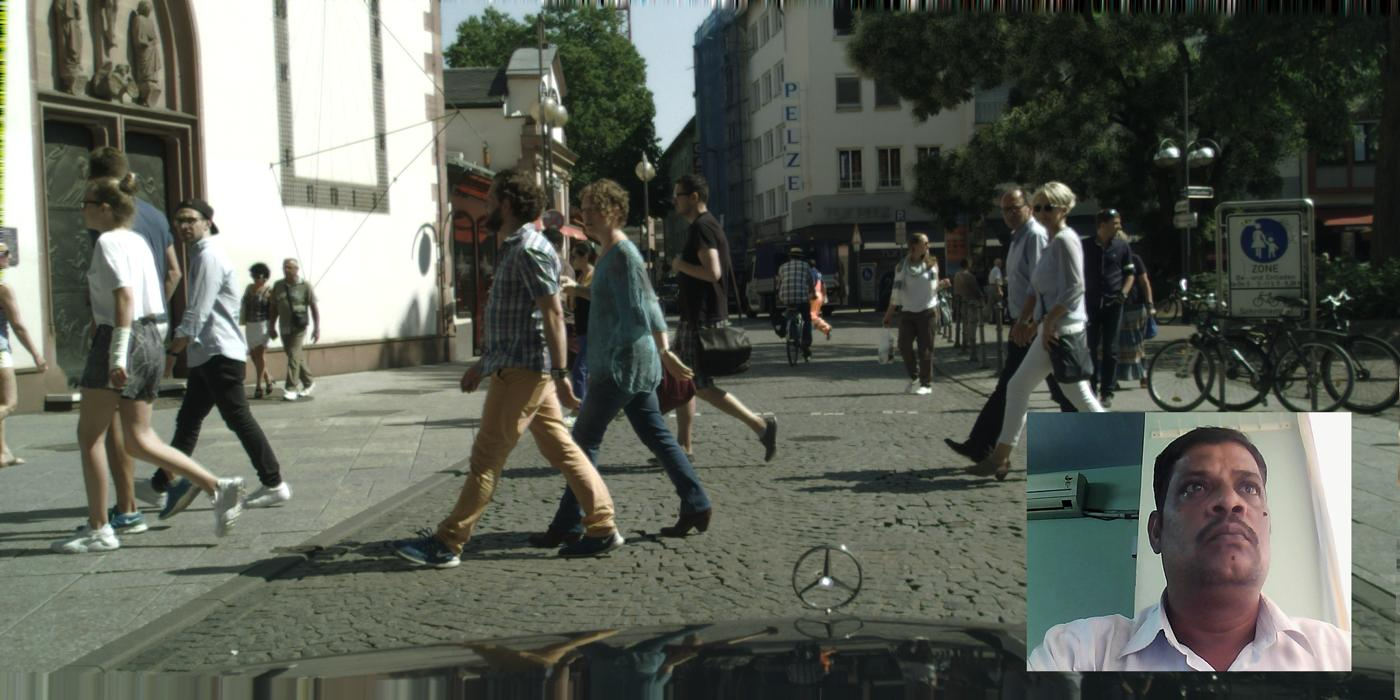
\includegraphics[width=0.23\linewidth]{frankfurt_000080_000029_leftImg8bit_modf.jpg}}
% \hspace{0.2cm}
% &
%                 \adjustbox{trim={.01\width} {.02\height} {0.01\width} {.02\height},clip}
%     {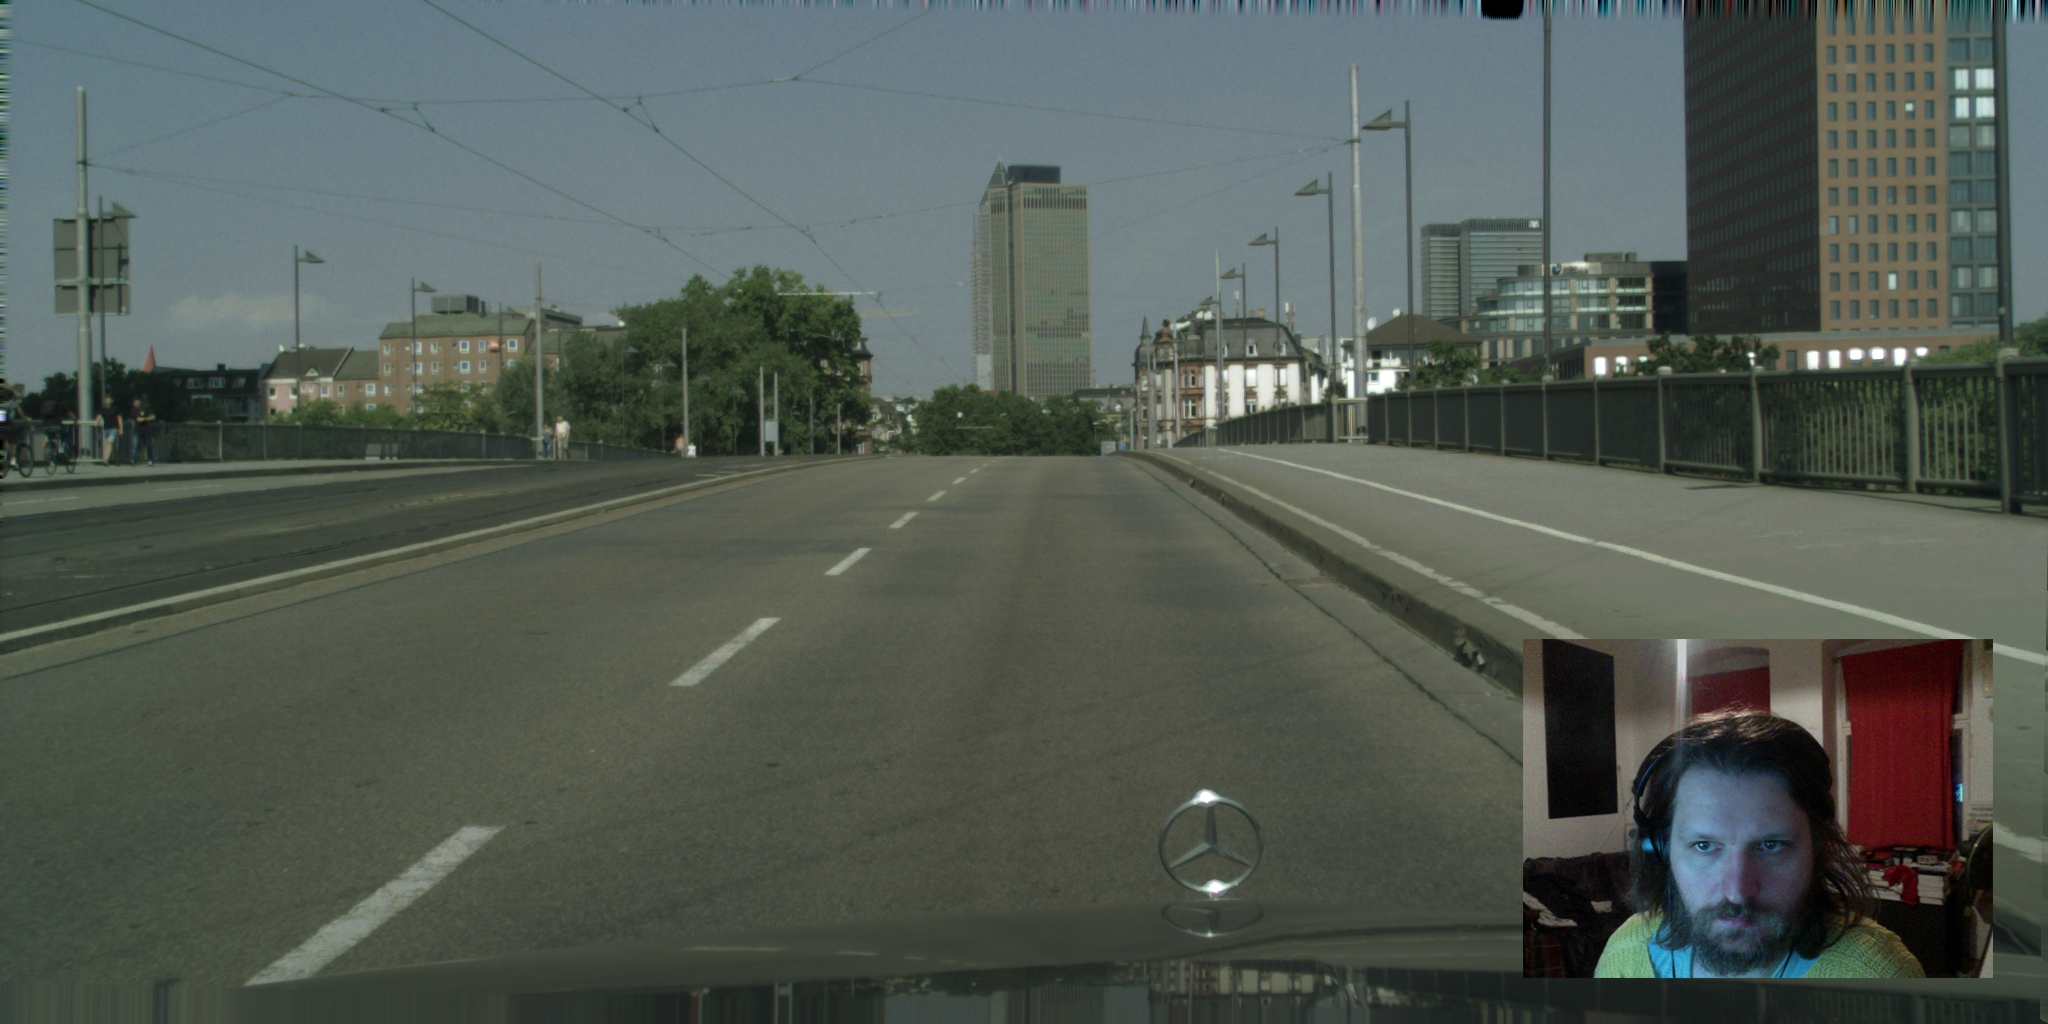
\includegraphics[width=0.23\linewidth]{frankfurt_000019_000029_leftImg8bit_modf.jpg}}
%     \\
%     \begin{turn}{90}{\scriptsize Intermediate Results}\end{turn}
% %    \multicolumn{3}{c}{\tiny a huge car is turning right side of the road near the building area}\\
%    % \vspace{0.02cm}
%    &
%   \adjustbox{trim={.08\width} {.22\height} {0.11\width} {.18\height},clip}
%     {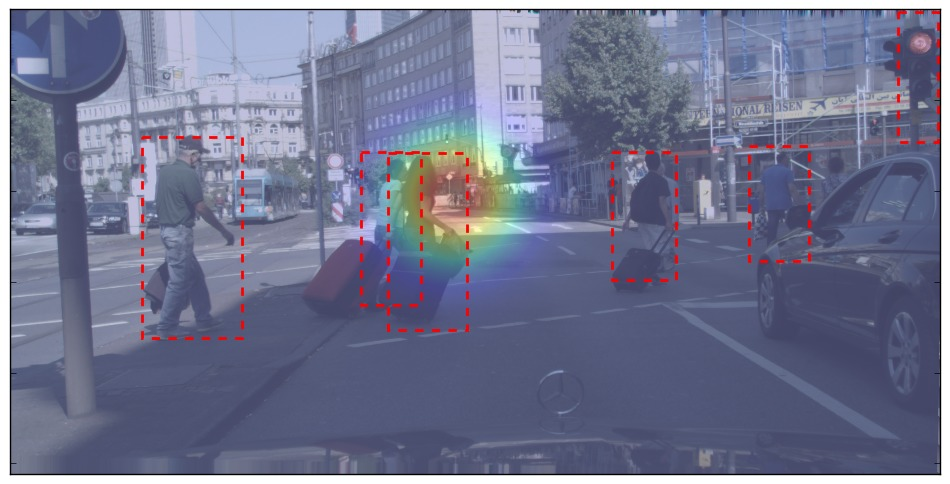
\includegraphics[width=0.3\linewidth]{demo_140_0.jpg}}
% \noindent &
% \adjustbox{trim={.08\width} {.22\height} {0.11\width} {.18\height},clip}
%     {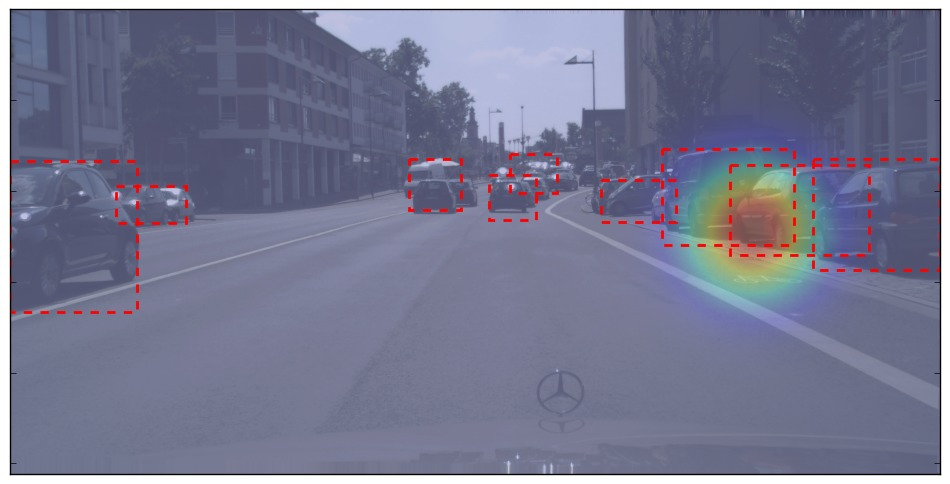
\includegraphics[width=0.3\linewidth]{demo_208_0.jpg}}
%     &
%     \adjustbox{trim={.08\width} {.22\height} {0.11\width} {.18\height},clip}
%     {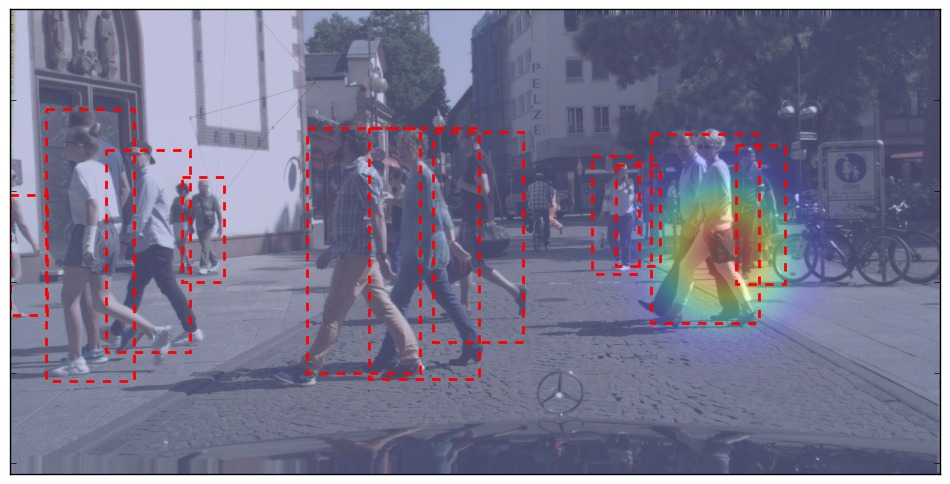
\includegraphics[width=0.3\linewidth]{demo_80_0.jpg}}
%     &
%     \adjustbox{trim={.08\width} {.22\height} {0.11\width} {.18\height},clip}
%     {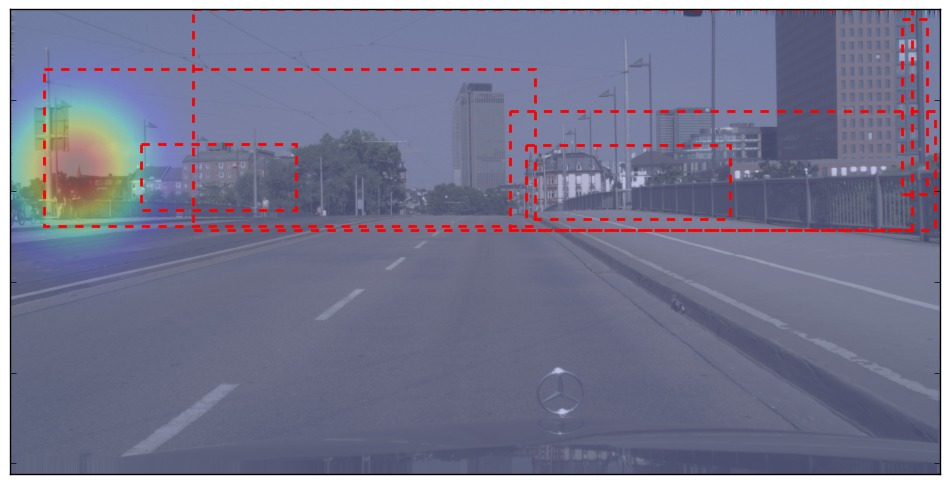
\includegraphics[width=0.3\linewidth]{demo_19_0.jpg}}
%     \\
%     \begin{turn}{90}{\scriptsize Final Results}\end{turn}
% %    \multicolumn{3}{c}{\tiny a car is parked on the right side of the road in front of a bike}\\
%        &  \adjustbox{trim={.08\width} {.22\height} {0.11\width} {.18\height},clip}
%     {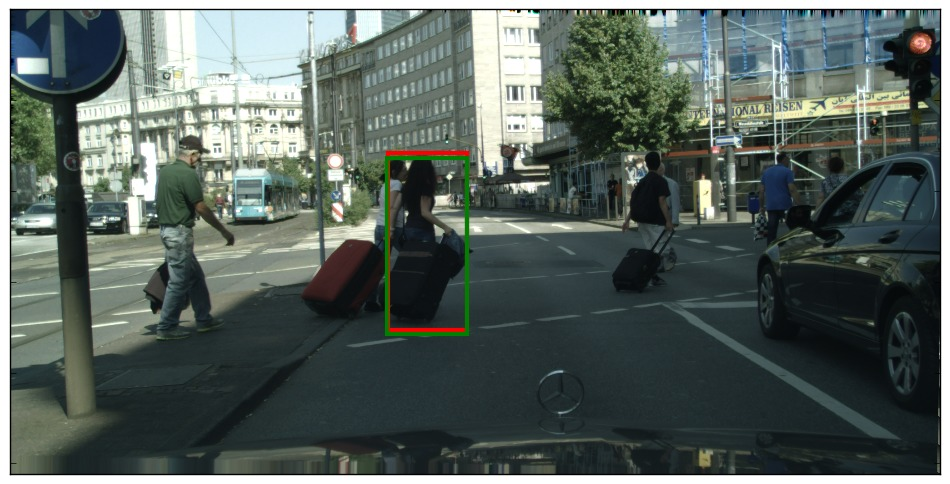
\includegraphics[width=0.3\linewidth]{rdemo_140_0.jpg}}
% \noindent 
% & \adjustbox{trim={.08\width} {.22\height} {0.11\width} {.18\height},clip}
%     {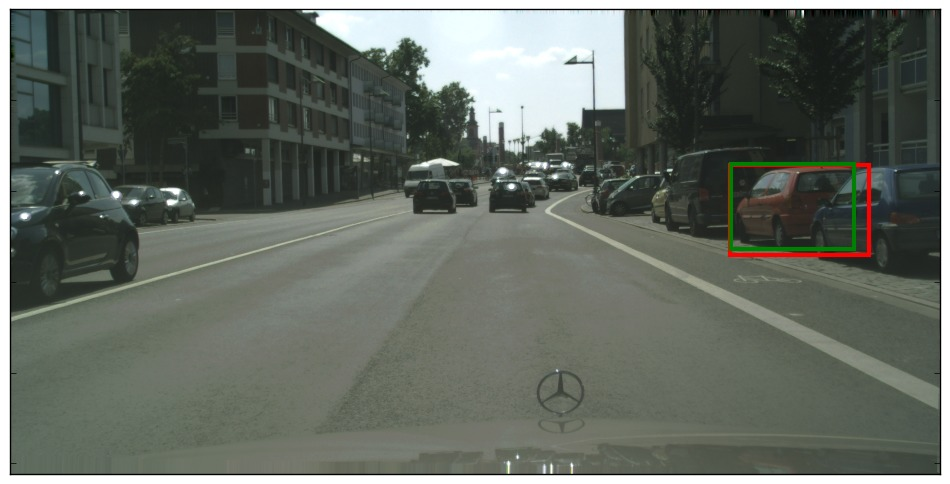
\includegraphics[width=0.3\linewidth]{rdemo_208_0.jpg}}
%     &
%     \adjustbox{trim={.08\width} {.22\height} {0.11\width} {.18\height},clip}
%     {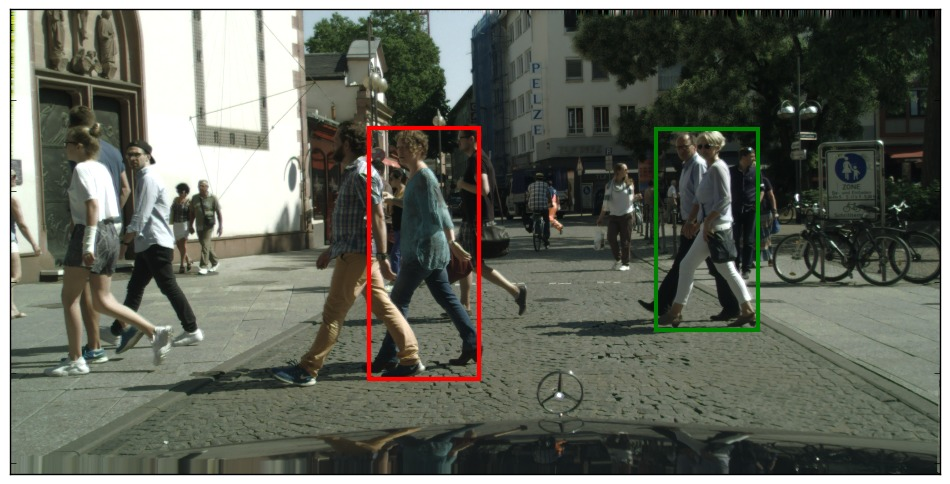
\includegraphics[width=0.3\linewidth]{rdemo_80_0.jpg}}
%     &    \adjustbox{trim={.08\width} {.22\height} {0.11\width} {.18\height},clip}
%     {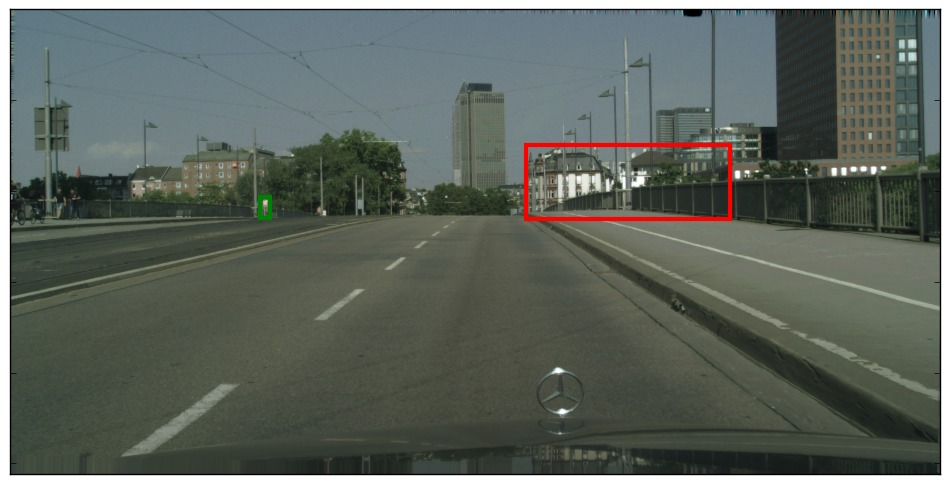
\includegraphics[width=0.3\linewidth]{rdemo_19_0.jpg}} \\
% %\noindent 
% %\includegraphics[width=0.5\linewidth]{Recall-IoU-100proposals.jpg}
% %\noindent 
% %\includegraphics[width=0.5\linewidth]{Recall-Candidates-IoU_0_9.jpg}
% \end{tabular}
% \caption{We show inputs on the first row. Middle row represents intermediate results where Gaze estimation is embedded on the image with object proposals while bottom row represents the final object localization results. These results are obtained on the Cityscape dataset.  {\color{green} Green} boxes represents ground truth box and {\color{red}Red} boxes represent proposals and the predicted boxes.}
% \label{fig:qual-gaze-results-cityscape}
% \end{figure*}

\noindent
\textbf{Qualitative Results}.
We provide some qualitative results in Fig.~\ref{fig:qual-gaze-results-cityscape}. Top row represents the inputs including video sequence from Cityscapes, gaze recording video and the referring expression. Having overlaid the gaze estimate over object proposals (middle row), we can also observe the proximity of the gaze estimate to the referred objects. We show the predicted and groundtruth box in the bottom row. We add also some failure cases in Fig.~\ref{fig:qual-gaze-results-cityscape}. From the above experiments, we infer that use of multi modal inputs - depth features, motion features, and speaker's gaze, along with RGB image features - improves the performance of object referring. 

%It is very intuitive that referring expressions that describe  motion are better addressed when we use motion cues. 

% \vspace{-4pt}
% \item 
% Cues from the Gaze significantly improves the object localization. Max pooling of object features seems to be better performer than averaging as max operation reduce the discrepancy in gaze estimation over the video. This can be inferred from Tab.~\ref{tab:gaze-comparison}. Even in real scenarios, gaze at an object can be instantaneous before referring them. Hence, max pooling seems to a better choice to capture the gaze feature even for the instantaneous case.
% %With the use of LOP, we generate sample dependent object proposals instead of fixed numbers of object proposals. Thus, LOP keeps a check on passing poor candidate proposals to TSCRC model. 
% %As a future work, we plan to explore minimal number of query specific object proposals for the object detection task.  
% \end{enumerate}ort forwarding for your router.

\section{Conclusions} 
\label{sec:conclusion}

In this work, we have proposed a solution for object referring (OR) in videos using language and gaze. The main contributions are made by the work: 1) we have developed a new video OR dataset with $30,000$ objects annotated across $5,000$ different video sequences; 2) we have developed a novel approach Temporal-Spatial Context Recurrent ConvNet for OR in videos, which integrated appearance, motion, depth, human gaze and spatio-temporal contextual information that can be trained in an end-to-end fashion; and 3) We have recorded gaze on all the annotated objects for the above dataset and showed the effectiveness of gaze for OR. 
%We believe that video OR dataset will spark more research interest in this direction. 
Experiments show that our model can effectively utilize motion cues, gaze cues and spatio-temporal context information provided by stereo videos outperforming image-based OR methods consistently. Training and evaluating our method, especially the contribution of the multiple modalities, in a real human-to-robot communication system constitute our future work. 
%We have also shown that Gaze help TSCRC favorably to improve the LOR task.  The dataset and code will be made available. 

\noindent
\textbf{Acknowledgement}: The work is supported by Toyota via the research project TRACE-Zurich.  

{\small
\bibliographystyle{ieee}
\bibliography{egbib}
}

\end{document}
